% \documentclass{extarticle}
% \usepackage[T2A]{fontenc}
% \usepackage[utf8]{inputenc}
% \usepackage[russian]{babel}
% \usepackage{titlesec}
% \title{пример с приложениями}
% \begin{document}
% \section{раз}
% текст
% \section{два}
% текст
% \appendix
% \titleformat{\section}[display]
%   {\normalfont\Large\bfseries}
%   {\centering Приложение\ \thesection\\(справочное)}
%   {0pt}{\Large\centering}
% \renewcommand{\thesection}{\Asbuk{section}}

% \section{приложение раз}
% текст
% \section{приложение два}
% текст
% \end{document}

% !TeX spellcheck = russian-aot-ieyo
% Зачем: Определяет класс документа (То, как будет выглядеть документ)
% Примечание: параметр draft помечает строки, вышедшие за границы страницы, прямоугольником, в финальной версии его нужно удалить.
\documentclass[a4paper,14pt,russian,oneside,final]{extreport}

% Зачем: Выбор внутренней TeX кодировки.
\usepackage[T2A]{fontenc}

% Зачем: Предоставляет свободный Times New Roman.
% Шрифт идёт вместе с пакетом scalable-cyrfonts-tex в Ubuntu/Debian

% пакет scalable-cyrfonts-tex может конфликтовать с texlive-fonts-extra в Ubuntu
% решение: Для себя я решил эту проблему так: пересобрал пакет scalable-cyrfonts-tex, изменив его имя. Решение топорное, но работает. Желающие могут скачать мой пакет здесь:
% https://yadi.sk/d/GW2PhDgEcJH7m
% Установка:
% dpkg -i scalable-cyrfonts-tex-shurph_4.16_all.deb

\usefont{T2A}{ftm}{m}{sl}
% не забудьте закомментировать \input{fonts_windows}

% Зачем: Установка кодировки исходных файлов.
\usepackage[utf8]{inputenc}

% Зачем: Делает результирующий PDF "searchable and copyable".
\usepackage{cmap}

\usepackage{titlesec}

% Зачем: Учет особенностей различных языков.
\usepackage[russian]{babel}

% Зачем: Добавляет поддержу дополнительных размеров текста 8pt, 9pt, 10pt, 11pt, 12pt, 14pt, 17pt, and 20pt.
% Почему: Пункт 2.1.1 Требований по оформлению пояснительной записки.
\usepackage{extsizes}

\usepackage[autostyle]{csquotes}

% Зачем: Длинна, пимерно соответвующая 5 символам
% Почему: Требования содержат странное требование про отсупы в 5 символов (для немоноширинного шрифта :| )
\newlength{\fivecharsapprox}
\setlength{\fivecharsapprox}{6ex}

\newcommand{\emptysection}[0]{{}}

\newcommand{\BeginAppendices}[0]{%
  \setcounter{section}{0}%
  \setcounter{figure}{0}%
  \renewcommand{\thesection}{\Asbuk{section}}%
}

\newcommand{\appendice}[1]{%
  \stepcounter{section}%
  \emptysection%
  \begin{center}%
  \textbf{\MakeUppercase{Приложение \thesection} \\ (обязательное)\\#1}%
  \end{center}%
  \addcontentsline{toc}{section}{Приложение \thesection}%
}

% Зачем: Добавляет отступы для абзацев.
% Почему: Пункт 2.1.3 Требований по оформлению пояснительной записки.
\usepackage{indentfirst}
\setlength{\parindent}{\fivecharsapprox} % Примерно соответсвует 5 символам.
\usepackage{float}


% Зачем: Настраивает отступы от границ страницы.
% Почему: Пункт 2.1.2 Требований по оформлению пояснительной записки.
% \usepackage[left=2.7cm,top=1.8cm,right=1.7cm,bottom=1.8cm]{geometry} % (1)
\usepackage[left=2.9cm,top=1.9cm,right=1.5cm,bottom=1.9cm]{geometry} % (2) -- стандарт
% \usepackage[left=2.7cm,top=1.3cm,right=1.2cm,bottom=1.2cm]{geometry} % (3)
% \usepackage[left=2.8cm,top=1.3cm,right=1.0cm,bottom=1.0cm]{geometry} % (4)


% Зачем: Настраивает межстрочный интервал, для размещения 40 +/- 3 строки текста на странице.
% Почему: Пункт 2.1.1 Требований по оформлению пояснительной записки.
\usepackage[nodisplayskipstretch]{setspace} 
\setstretch{1.2}
%\onehalfspacing

% Зачем: Выбор шрифта по-умолчанию. 
% Почему: Пункт 2.1.1 Требований по оформлению пояснительной записки.
% Примечание: В требованиях не указан, какой именно шрифт использовать. По традиции используем TNR.
\renewcommand{\rmdefault}{cmr} % Times New Roman


% Зачем: Отключает использование изменяемых межсловных пробелов.
% Почему: Так не принято делать в текстах на русском языке.
\frenchspacing


% Зачем: Сброс счетчика сносок для каждой страницы
% Примечание: в "Требованиях по оформлению пояснительной записки" не указано, как нужно делать, но в других БГУИРовских докуметах рекомендуется нумерация отдельная для каждой страницы
\usepackage{perpage}
\MakePerPage{footnote}

% Зачем: Добавляет скобку 1) к номеру сноски
% Почему: Пункты 2.9.2 и 2.9.1 Требований по оформлению пояснительной записки.
\makeatletter 
\def\@makefnmark{\hbox{\@textsuperscript{\normalfont\@thefnmark)}}}
\makeatother


% Зачем: Расположение сносок внизу страницы
% Почему: Пункт 2.9.2 Требований по оформлению пояснительной записки.
\usepackage[bottom]{footmisc}


% Зачем: Переопределяем стандартную нумерацию, т.к. в отчете будут только section и т.д. в терминологии TeX
\makeatletter
\renewcommand{\thesection}{\arabic{section}}
\makeatother


% Зачем: Пункты (в терминологии требований) в терминологии TeX subsubsection должны нумероваться
% Почему: Пункт 2.2.3 Требований по оформлению пояснительной записки.
\setcounter{secnumdepth}{3}


% Зачем: Настраивает отступ между таблицей с содержанимем и словом СОДЕРЖАНИЕ
% Почему: Пункт 2.2.7 Требований по оформлению пояснительной записки.
\usepackage{tocloft}
\setlength{\cftbeforetoctitleskip}{-1em}
\setlength{\cftaftertoctitleskip}{1em}


% Зачем: Определяет отступы слева для записей в таблице содержания.
% Почему: Пункт 2.2.7 Требований по оформлению пояснительной записки.
\makeatletter
\renewcommand{\l@section}{\@dottedtocline{1}{0.5em}{1.2em}}
\renewcommand{\l@subsection}{\@dottedtocline{2}{1.7em}{2.0em}}
\makeatother

% Зачем: убираем переносы в содержании
\makeatletter
\renewcommand{\@tocrmarg}{\@pnumwidth plus1fil}
\makeatother


% Зачем: Работа с колонтитулами
\usepackage{fancyhdr} % пакет для установки колонтитулов
\pagestyle{fancy} % смена стиля оформления страниц


% Зачем: Нумерация страниц располагается справа снизу страницы
% Почему: Пункт 2.2.8 Требований по оформлению пояснительной записки.
\fancyhf{} % очистка текущих значений
\fancyfoot[R]{\thepage} % установка верхнего колонтитула
\renewcommand{\footrulewidth}{0pt} % убрать разделительную линию внизу страницы
\renewcommand{\headrulewidth}{0pt} % убрать разделительную линию вверху страницы
\fancypagestyle{plain}{ 
    \fancyhf{}
    \rfoot{\thepage}}
\setlength{\footskip}{6mm}


% Зачем: Задает стиль заголовков раздела жирным шрифтом, прописными буквами, без точки в конце
% Почему: Пункты 2.1.1, 2.2.5, 2.2.6 и ПРИЛОЖЕНИЕ Л Требований по оформлению пояснительной записки.
\makeatletter
\renewcommand\section{%
  \clearpage\@startsection {section}{1}%
    {\fivecharsapprox}%
    {-1em \@plus -1ex \@minus -.2ex}%
    {1em \@plus .2ex}%
    {\raggedright\hyphenpenalty=10000\normalfont\bfseries\MakeUppercase}}
\makeatother


% Зачем: Задает стиль заголовков подразделов
% Почему: Пункты 2.1.1, 2.2.5 и ПРИЛОЖЕНИЕ Л Требований по оформлению пояснительной записки.
% \makeatletter
% \renewcommand\subsection{%
%   \@startsection{subsection}{2}%
%     {\fivecharsapprox\bfseries}%
%     {-1em \@plus -1ex \@minus -.2ex}%
%     {1em \@plus .2ex}%
%     {\raggedright\hyphenpenalty=10000\normalfont\normalsize}}
% \makeatother

% Полужирным и номер, и текст заголовка (если ваша кафедра не ПОИТ)
\makeatletter
\renewcommand\subsection{%
  \@startsection{subsection}{2}%
    {\fivecharsapprox}%
    {-1em \@plus -1ex \@minus -.2ex}%
    {1em \@plus .2ex}%
    {\raggedright\hyphenpenalty=10000\normalfont\normalsize\bfseries}}
\makeatother


% Зачем: Задает стиль заголовков пунктов
% Почему: Пункты 2.1.1, 2.2.5 и ПРИЛОЖЕНИЕ Л Требований по оформлению пояснительной записки.
\makeatletter
\renewcommand\subsubsection{
  \@startsection{subsubsection}{3}%
    {\fivecharsapprox\bfseries}%
    {-1em \@plus -1ex \@minus -.2ex}%
    {\z@}%
    {\raggedright\hyphenpenalty=10000\normalfont\normalsize}}
\makeatother

% Зачем: для оформления введения и заключения, они должны быть выровнены по центру.
% Почему: Пункты 1.1.15 и 1.1.11 Требований по оформлению пояснительной записки.
\makeatletter
\newcommand\sectioncentered{%
  \clearpage\@startsection {section}{1}%
    {\z@}%
    {-1em \@plus -1ex \@minus -.2ex}%
    {1em \@plus .2ex}%
    {\centering\hyphenpenalty=10000\normalfont\bfseries\MakeUppercase}%
    }
\makeatother



% Зачем: Задает стиль библиографии
% Почему: Пункт 2.8.6 Требований по оформлению пояснительной записки.
\bibliographystyle{styles/belarus-specific-utf8gost780u}


% Зачем: Пакет для вставки картинок
% Примечание: Объяснение, зачем final - http://tex.stackexchange.com/questions/11004/why-does-the-image-not-appear
\usepackage[final]{graphicx}
\DeclareGraphicsExtensions{.pdf,.png,.jpg,.eps}


% Зачем: Директория в которой будет происходить поиск картинок
\graphicspath{{attachments/}}


% Зачем: Добавление подписей к рисункам
\usepackage[nooneline]{caption}
\usepackage{subcaption}

% Зачем: чтобы работала \No в новых латехах
\DeclareRobustCommand{\No}{\ifmmode{\nfss@text{\textnumero}}\else\textnumero\fi}

% зачем: sidewaysfigure для поворота рисунков
\usepackage{rotating}
% Зачем: поворот ячеек таблиц на 90 градусов
\DeclareRobustCommand{\povernut}[1]{\begin{sideways}{#1}\end{sideways}}


% Зачем: заставляем работать ссылки (\footnote) в таблицах
\usepackage{tablefootnote}



% Зачем: когда в формулах много кириллических символов команда \text{} занимает много места
\DeclareRobustCommand{\x}[1]{\text{#1}}


% Зачем: Задание подписей, разделителя и нумерации частей рисунков
% Почему: Пункт 2.5.5 Требований по оформлению пояснительной записки.
\DeclareCaptionLabelFormat{stbfigure}{Рисунок #2}
\DeclareCaptionLabelFormat{stbsubfigure}{#2}
\DeclareCaptionLabelFormat{stbtable}{Таблица #2}
\DeclareCaptionLabelSeparator{stb}{~--~}
\DeclareCaptionLabelSeparator{stbsubfiguresep}{)~}
\captionsetup{labelsep=stb}
\captionsetup[subfigure]{labelformat=stbsubfigure,labelsep=stbsubfiguresep}
\captionsetup[figure]{labelformat=stbfigure,justification=centering,skip=15pt}
\captionsetup[table]{labelformat=stbtable,justification=raggedright,format=hang,skip=0pt}
\renewcommand{\thesubfigure}{\asbuk{subfigure}}


% Зачем: Окружения для оформления формул
% Почему: Пункт 2.4.7 требований по оформлению пояснительной записки и специфические требования различных кафедр
\usepackage{calc}
\newlength{\lengthWordWhere}
\settowidth{\lengthWordWhere}{где}
\newenvironment{explanationx}
    {%
    %%% Следующие строки определяют специфические требования разных редакций стандартов. Раскоменнтируйте нужную строку
    %% стандартный абзац, СТП-01 2010
    %\begin{itemize}[leftmargin=0cm, itemindent=\parindent + \lengthWordWhere + \labelsep, labelsep=\labelsep]
    %% без отступа, СТП-01 2013
    \begin{itemize}[leftmargin=0cm, itemindent=\lengthWordWhere + \labelsep , labelsep=\labelsep]%
    \renewcommand\labelitemi{}%
    }
    {%
    %\\[\parsep]
    \end{itemize}
    }

% Старое окружение для "где". Сохранено для совместимости
\usepackage{tabularx}

\newenvironment{explanation}
    {
    %%% Следующие строки определяют специфические требования разных редакций стандартов. Раскоменнтируйте нужные 2 строки
    %% стандартный абзац, СТП-01 2010
    %\par 
    %\tabularx{\textwidth-\fivecharsapprox}{@{}ll@{ --- } X }
    %% без отступа, СТП-01 2013
    \noindent 
    \tabularx{\textwidth}{@{}ll@{ --- } X }
    }
    { 
    \\[\parsep]
    \endtabularx
    \vspace{-1.2em} % костыль, вдруг понадобится после "где"-области убрать пустую строку
    }


% Зачем: Удобная вёрстка многострочных формул, масштабирующийся текст в формулах, формулы в рамках и др
\usepackage{amsmath}


% Зачем: Поддержка ажурного и готического шрифтов 
\usepackage{amsfonts}


% Зачем: amsfonts + несколько сотен дополнительных математических символов
\usepackage{amssymb}


% Зачем: Окружения «теорема», «лемма»
\usepackage{amsthm}


% Зачем: Чтобы можно было использовать русские буквы в формулах, но в случае использования предупреждать об этом.
\usepackage[warn]{mathtext}


% Зачем: Производить арифметические операции во время компиляции TeX файла
\usepackage{calc}

% Зачем: Производить арифметические операции во время компиляции TeX файла
\usepackage{fp}

% Зачем: Пакет для работы с перечислениями
\usepackage{enumitem}
\makeatletter
 \AddEnumerateCounter{\asbuk}{\@asbuk}{щ)}
\makeatother


% Зачем: Устанавливает символ начала простого перечисления
% Почему: Пункт 2.3.5 Требований по оформлению пояснительной записки.
\setlist{nolistsep}


% Зачем: Устанавливает символ начала именованного перечисления
% Почему: Пункт 2.3.8 Требований по оформлению пояснительной записки.
\renewcommand{\labelenumi}{\asbuk{enumi})}
\renewcommand{\labelenumii}{\arabic{enumii})}
\renewcommand{\labelenumiii}{\Roman{enumiii})}

% Зачем: Устанавливает отступ от границы документа до символа списка, чтобы этот отступ равнялся отступу параграфа
% Почему: Пункт 2.3.5 Требований по оформлению пояснительной записки.

\setlist[itemize,0]{itemindent=\parindent + 2.2ex,leftmargin=0ex,label=--}
\setlist[enumerate,1]{itemindent=\parindent + 2.7ex,leftmargin=0ex}
\setlist[enumerate,2]{itemindent=\parindent + \parindent - 2.7ex}
\setlist[enumerate,3]{itemindent=\parindent + \parindent - 2.7ex}

% Зачем: Включение номера раздела в номер формулы. Нумерация формул внутри раздела.
\AtBeginDocument{\numberwithin{equation}{section}}

% Зачем: Включение номера раздела в номер таблицы. Нумерация таблиц внутри раздела.
\AtBeginDocument{\numberwithin{table}{section}}

% Зачем: Включение номера раздела в номер рисунка. Нумерация рисунков внутри раздела.
\AtBeginDocument{\numberwithin{figure}{section}}


% Зачем: Дополнительные возможности в форматировании таблиц
\usepackage{makecell}
\usepackage{multirow}
\usepackage{array, booktabs}


% Зачем: "Умная" запятая в математических формулах. В дробных числах не добавляет пробел
% Почему: В требованиях не нашел, но в русском языке для дробных чисел используется {,} а не {.}
\usepackage{icomma}

% Зачем: макрос для печати римских чисел
\makeatletter
\newcommand{\rmnum}[1]{\romannumeral #1}
\newcommand{\Rmnum}[1]{\expandafter\@slowromancap\romannumeral #1@}
\makeatother


% Зачем: Управление выводом чисел.
\usepackage{sistyle}
\SIdecimalsign{,}

% Зачем: inline-коментирование содержимого.
\newcommand{\ignore}[2]{\hspace{0in}#2}


% Зачем: Возможность коментировать большие участки документа
\usepackage{verbatim}


\usepackage{xcolor}


% Зачем: Оформление листингов кода
% Примечание: final нужен для переопределения режима draft, в котором листинги не выводятся в документ.
\usepackage[final]{listings}


% Зачем: настройка оформления листинга для языка F#
\definecolor{bluekeywords}{rgb}{0.13,0.13,1}
\definecolor{greencomments}{rgb}{0,0.5,0}
\definecolor{turqusnumbers}{rgb}{0.17,0.57,0.69}
\definecolor{redstrings}{rgb}{0.5,0,0}

\renewcommand{\lstlistingname}{Листинг}

\lstdefinelanguage{FSharp}
    {morekeywords={abstract,and,as,assert,base,begin,class,default,delegate,do,done,downcast,downto,elif,else,end,exception,extern,false,finally,for,fun,function,global,if,in,inherit,inline,interface,internal,lazy,let,let!,match,member,module,mutable,namespace,new,not,null,of,open,or,override,private,public,rec,return,return!,select,static,struct,then,to,true,try,type,upcast,use,use!,val,void,when,while,with,yield,yield!,asr,land,lor,lsl,lsr,lxor,mod,sig,atomic,break,checked,component,const,constraint,constructor,continue,eager,event,external,fixed,functor,include,method,mixin,object,parallel,process,protected,pure,sealed,tailcall,trait,virtual,volatile},
    keywordstyle=\bfseries\color{bluekeywords},
    sensitive=false,
    morecomment=[l][\color{greencomments}]{///},
    morecomment=[l][\color{greencomments}]{//},
    morecomment=[s][\color{greencomments}]{{(*}{*)}},
    morestring=[b]",
    stringstyle=\color{redstrings},
    }

\lstdefinestyle{fsharpstyle}{
   xleftmargin=0ex,
   language=FSharp,
   basicstyle=\footnotesize\ttfamily,
   breaklines=true,
   columns=fullflexible
}

\lstdefinestyle{csharpinlinestyle} {
  language=[Sharp]C,
  morekeywords={yield,var,get,set,from,select,partial,where,async,await},
  breaklines=true,
  columns=fullflexible,
  basicstyle=\footnotesize\ttfamily
}

\lstdefinestyle{python}{
   xleftmargin=0ex,
   language=Python,
   basicstyle=\footnotesize\ttfamily,
   breaklines=true,
   columns=fullflexible
}

\lstdefinestyle{sql}{
   xleftmargin=0ex,
   language=SQL,
   basicstyle=\footnotesize\ttfamily,
   breaklines=true,
   columns=fullflexible
}

\lstdefinestyle{csharpstyle}{
   xleftmargin=0ex,
   language=[Sharp]C,
   basicstyle=\footnotesize\ttfamily,
   breaklines=true,
   columns=fullflexible
}

\definecolor{lightgray}{rgb}{.9,.9,.9}
\definecolor{darkgray}{rgb}{.4,.4,.4}
\definecolor{purple}{rgb}{0.65, 0.12, 0.82}
\definecolor{white}{rgb}{1, 1, 1}

\lstdefinelanguage{JavaScript}{
  keywords={break, case, catch, continue, debugger, default, delete, do, else, false, finally, for, function, if, in, instanceof, new, null, return, switch, this, throw, true, try, typeof, var, void, while, with},
  morecomment=[l]{//},
  morecomment=[s]{/*}{*/},
  morestring=[b]',
  morestring=[b]",
  ndkeywords={class, export, boolean, throw, implements, import, this},
  keywordstyle=\color{blue}\bfseries,
  ndkeywordstyle=\color{darkgray}\bfseries,
  identifierstyle=\color{black},
  commentstyle=\color{purple}\ttfamily,
  stringstyle=\color{red}\ttfamily,
  sensitive=true
}

\lstdefinestyle{js}{
   xleftmargin=0ex,
   language=JavaScript,
   basicstyle=\footnotesize\ttfamily,
   breaklines=true,
   columns=fullflexible
}

\definecolor{keyword}{HTML}{BA2CA3}
\definecolor{string}{HTML}{D12F1B}
\definecolor{comment}{HTML}{008400}

\lstdefinestyle{swiftStyle} {
	xleftmargin=0ex,
   language=swift,
   basicstyle=\footnotesize\ttfamily,
   breaklines=true,
   columns=fullflexible
}
\lstdefinelanguage{swift}
{
  morekeywords={
    func,if,then,else,for,in,while,do,switch,case,default,where,break,continue,fallthrough,return,
    typealias,struct,class,enum,protocol,var,func,let,get,set,willSet,didSet,inout,init,deinit,extension,
    subscript,prefix,operator,infix,postfix,precedence,associativity,left,right,none,convenience,dynamic,
    final,lazy,mutating,nonmutating,optional,override,required,static,unowned,safe,weak,internal,
    private,public,is,as,self,unsafe,dynamicType,true,false,nil,Type,Protocol,fileprivate,import,
  },
  morecomment=[l]{//}, % l is for line comment
  morecomment=[s]{/*}{*/}, % s is for start and end delimiter
  morestring=[b]" % defines that strings are enclosed in double quotes
}



\lstset{
  language=swift,
  backgroundcolor=\color{white},
  extendedchars=true,
  basicstyle=\small\ttfamily,
  showstringspaces=false, % lets spaces in strings appear as real spaces
  columns=fixed,
  keepspaces=true,
  keywordstyle=\color{keyword},
  stringstyle=\color{string},
  commentstyle=\color{comment},
   numberstyle=\footnotesize,
  showspaces=false,
   numbersep=9pt,
   tabsize=4,
   breaklines=true,
   showtabs=false,
   captionpos=b
  numbers=none
}

% Зачем: Нумерация листингов в пределах секции
\AtBeginDocument{\numberwithin{lstlisting}{section}}

\usepackage[normalem]{ulem}

\usepackage[final,hidelinks]{hyperref}
% Моноширинный шрифт выглядит визуально больше, чем пропорциональный шрифт, если их размеры одинаковы. Искусственно уменьшаем размер ссылок.
\renewcommand{\UrlFont}{\small\rmfamily\tt}

\usepackage[square,numbers,sort&compress]{natbib}
\setlength{\bibsep}{0em}

% Магия для подсчета разнообразных объектов в документе
\usepackage{totcount}
\regtotcounter{section}

\usepackage{etoolbox}

\newcounter{totfigures}
\newcounter{tottables}
\newcounter{totreferences}
\newcounter{totequation}

\providecommand\totfig{} 
\providecommand\tottab{}
\providecommand\totref{}
\providecommand\toteq{}

\makeatletter
\AtEndDocument{%
  \addtocounter{totfigures}{\value{figure}}%
  \addtocounter{tottables}{\value{table}}%
  \addtocounter{totequation}{\value{equation}}
  \immediate\write\@mainaux{%
    \string\gdef\string\totfig{\number\value{totfigures}}%
    \string\gdef\string\tottab{\number\value{tottables}}%
    \string\gdef\string\totref{\number\value{totreferences}}%
    \string\gdef\string\toteq{\number\value{totequation}}%
  }%
}
\makeatother

\pretocmd{\section}{\addtocounter{totfigures}{\value{figure}}\setcounter{figure}{0}}{}{}
\pretocmd{\section}{\addtocounter{tottables}{\value{table}}\setcounter{table}{0}}{}{}
\pretocmd{\section}{\addtocounter{totequation}{\value{equation}}\setcounter{equation}{0}}{}{}
\pretocmd{\bibitem}{\addtocounter{totreferences}{1}}{}{}

% Для оформления таблиц, не влазящих на 1 страницу
\usepackage{longtable}

% Для использования знака градуса и других знаков
% http://ctan.org/pkg/gensymb
\usepackage{textcomp}
\usepackage{gensymb}

% Зачем: преобразовывать текст в верхний регистр командой MakeTextUppercase
\usepackage{textcase}

% Зачем: Переносы в словах с тире.
% Тире в словае заменяем на \hyph: аппаратно\hyphпрограммный.
% https://stackoverflow.com/questions/2193307/how-to-get-latex-to-hyphenate-a-word-that-contains-a-dash#
\def\hyph{-\penalty0\hskip0pt\relax}

% Добавляем абзацный отступ для библиографии
% https://github.com/mstyura/bsuir-diploma-latex/issues/19
\setlength\bibindent{-1.0900cm}

\makeatletter
\renewcommand\NAT@bibsetnum[1]{\settowidth\labelwidth{\@biblabel{#1}}%
   \setlength{\leftmargin}{\bibindent}\addtolength{\leftmargin}{\dimexpr\labelwidth+\labelsep\relax}%
   \setlength{\itemindent}{-\bibindent+\fivecharsapprox-0.240cm}%
   \setlength{\listparindent}{\itemindent}
\setlength{\itemsep}{\bibsep}\setlength{\parsep}{\z@}%
   \ifNAT@openbib
     \addtolength{\leftmargin}{\bibindent}%
     \setlength{\itemindent}{-\bibindent}%
     \setlength{\listparindent}{\itemindent}%
     \setlength{\parsep}{10pt}%
   \fi
}

% Зачем: изменение ориентации отдельных страниц.
% Использование:
% \begin{landscape}
% ...
% \end{landscape}
\usepackage{lscape}

% Зачем: одноименную команду нужно писать в конце 
% макросов, чтобы компенсировать съедаемый латехом
% пробел (там где нужно).
\usepackage{xspace}

% Зачем: если таблица или рисунок находится на отдельной странице,
% то они должны находиться у верхнего края листа.
\makeatletter
\setlength{\@fptop}{0pt}
\setlength{\@fpbot}{0pt plus 1fil}
\makeatother

% Чтобы посчитать общее число страниц.
\usepackage{lastpage,refcount}

\newcommand{\csharp}{Swift\xspace}
\newcommand{\dotnet}{Microsoft .NET\xspace}
\newcommand{\typescript}{Ty\-pe\-Script\xspace}
\newcommand{\js}{Ja\-va\-Script\xspace}
\newcommand{\react}{React\xspace}
\newcommand{\mobx}{MobX\xspace}
\newcommand{\webpack}{Webpack\xspace}
\newcommand{\uml}{UML~2.1\xspace}
\newcommand{\nezaboodka}{Firebase Database\xspace}
\newcommand{\realm}{Realm\xspace}

\newcommand{\sourcecodeappendix}{А\xspace}
\newcommand{\dbschemeappendix}{Б\xspace}
\newcommand{\configfilesappendix}{В\xspace}


\begin{document}

% Initial

\begin{titlepage}
  \begin{center}
    Министерство образования Республики Беларусь\\[1em]
    Учреждение образования\\
    БЕЛОРУССКИЙ ГОСУДАРСТВЕННЫЙ УНИВЕРСИТЕТ \\
    ИНФОРМАТИКИ И РАДИОЭЛЕКТРОНИКИ\\[1em]

    \begin{minipage}{\textwidth}
      \begin{flushleft}
          Инженерно-экономический факультет\\
          Кафедра экономической информатики\\
      \end{flushleft}
    \end{minipage}\\[3.5em]

    {ПОЯСНИТЕЛЬНАЯ ЗАПИСКА}\\
    {к дипломному проекту}\\
    {на тему}\\[3em]
    \textbf{\large\MakeUppercase{Интернет вещей и программная поддержка управления адресной светодиодной лентой}}\\[1em]


    {БГУИР ДП  1-40 04 01 00 054 ПЗ}\\[2em]
    
    \begin{tabular}{ p{0.65\textwidth}p{0.25\textwidth} }
      Студент & Я.\,А.~Шнайдер \\
      Руководитель & Т.\,М.~Унучек
    \end{tabular}
    
    \vfill
    {\normalsize Минск 2019}
  \end{center}
\end{titlepage}


\newpage
\pagebreak
\thispagestyle{plain}
\setcounter{page}{4}

% Зачем: чтобы не было большого вертикального отступа сверху.
\setlength{\cftbeforetoctitleskip}{-2.9em}

% Зачем: Содержание пишется полужирным шрифтом, по центру всеми заглавными буквами
% Почему: Пункт 2.2.7 Требований по оформлению пояснительной записки.
\renewcommand \contentsname {\centerline{\textbf{\normalsize{\MakeUppercase{Содержание}}}}}

% Зачем: Не захламлять основной файл
{
\normalsize\selectfont
\tableofcontents
\newpage
}


% Sections

\sectioncentered*{Введение}
\addcontentsline{toc}{section}{Введение}
\label{sec:introduction}

Каждый новый год во многих уголках планеты люди начинают украшать свои дома и магазины различными новогодними игрушками. В том числе и гирляндами. И перед каждым человеком стоит вопрос: "Какие украшения мне стоит купить?". На этот вопрос сложно ответить, так как существует огромное множество различных новогодних украшений. Было бы намного удобней, если бы можно было купить одну гирлянду и настраивать ее под себя. Управление световыми эффектами представляет собой изменение цвета, скорости, создания собственных эффектов, применение предустановленных эффектов.

Перечисленные задачи особенно актуальны для предпринимателей: владельцев небольших магазинов, прилавков, а также различных торговых площадок. Так как именно они вынуждены привлекать потенциальных покупателей различными украшениями, а так же им может понадобиться изменять эффекты для того чтобы понять какие из них лучше влияют на количество покупателей. И людям для выполнения своих задач приходится комбинировать существующие гирлянды и приспосабливать их под свои нужды. Каждый человек вынужден тратить своё время на поиск украшений, тратить время на их конфигурирование. Это приводит к большим тратам, а так же возникает проблема с изменением анимаций уже после покупки.

Для задачи управления световыми эффектами реализовано не так много приложений для мобильных устройств, что благоприятно сказывается на конкурентоспособности приложения. В основном люди используют обычные гирлянды без возможности управления.

Целью настоящего курсового проекта является разработка программного средства, которое бы позволило как простым людям, так и предпринимателям, управлять световыми эффектами на гирляндах для украшения домов или привлечения внимания потенциальных покупателей. Также данный проект предоставляет возможность обмениваться созданными анимациями между пользователями. 

В пояснительной записке к курсовому проекту излагаются детали поэтапной разработки приложения управления световыми эффектами гирлянды.

\section{Описание предметной области}
\label{sec:analysis}

Кратко рассмотрим предметную область, задачи которой подлежат автоматизации в ходе выполнения курсового проекта.

Рассматриваемая предметная область – мобильное приложения для управления ``умной'' гирляндой. Основная задача предметной области – управление световым оборудованием в различных условиях.

Приложение для управления световым оборудованием (``умной'' гирляндой) представляет собой приложение, которое будет поставляться вместе с самим световым оборудованием. С помощью этого приложения, пользователь сможет управлять отображением различных анимаций на гирлянде (как заранее созданных, так и тех, что пользователь создал сам), калибровать приложение на основе текущего расположения гирлянды, чтобы большинство анимаций правильно отображались на ней. Также пользователь будет иметь возможность связывать несколько гирлянд в одну сеть, чтобы назначать им определенную последовательность из анимаций (проигрывать анимацию последовательно, от первой гирлянды к последней, либо отображать анимацию одновременно). Пользователь будет иметь гибкие возможности настройки каждой гирлянды (управление видимостью wi-fi модуля, имя wi-fi точки). Также будет реализована возможность пересылать самостоятельно созданные анимации другим людям, которые будут заригестрированы в приложении.


\subsection{Аналитический обзор литературных источников}
\label{sec:analysis:literature}

Далее приводится анализ сведений, которые влияют на формулирование требований, выбор архитектуры и дальнейшее проектирование и разработку программного средства.

\subsubsection{} Кроссплатформенность приложений
\label{sec:analysis:literature:crossplatform}

Как несколько десятилетий назад, так и в настоящее время выбор платформы является серьезным ограничением для всех последующих этапов разработки. Однако уже начали появляться технологии, которые позволяют использовать однажды написанный код на многих платформах. Сегодня все больше приложений создается сразу для нескольких платформ, а приложения, созданные изначально для одной платформы, активно адаптируются под другие. %\cite{habr_crossplatform}. 
Разработчик, изучающий какую-либо из таких технологий, получает конкурентное преимущество, поскольку за счет расширения количества платформ расширяется круг задач, над которыми он может работать. Поэтому кроссплатформенность -- реальная или потенциальная -- является одним из факторов, который необходимо учитывать при выборе технологий реализации проекта.

\subsubsection{} Обзор целевых платформ
\label{sec:analysis:literature:platforms}

Несмотря на планируемое использование кроссплатформенных технологий, поддержка всех платформ может затребовать значительно больших сред\-ств и времени, чем есть в наличии для выполнения дипломного проектирования. Поэтому, необходимо осуществить выбор одной основной платформы с расчетом на продолжение разработки и реализацию проекта для других платформ. Рассмотрим достоинства и недостатки основных.

\emph{Настольное приложение} – программное средство, которое запускает- ся локально на компьютере пользователя. При его создании появляется возможность использования всех преимуществ аппаратного обеспечения, которым оснащен компьютер, например: прямой доступ к видеокарте, внешним устройствам. Кроме того, появляется возможность взаимодействия с другими установленными приложениями.

Тем не менее у настольных приложений есть и ряд недостатков. Когда пользователь работает удаленно, возникают проблемы, связанные с сетью, соединениями, сетевыми экранами. Один из самых больших недостатков заключается в огромной сложности развертывания приложения на десятки или сотни машин, их конфигурирования, периодического обновления \cite{msdn_desktop_vs_web}.

\emph{Веб-приложения}, в отличие от настольных, работают на удаленном аппаратном обеспечении и поставляются пользователю через браузер \cite{web_based_vs_desktop}. При их использовании разработчик избавляется от необходимости поддерживать установку большого числа зависимостей, он всегда может быть уверен, что все пользователи используют самую последнюю версию приложения. Вычислительные операции могут производиться на мощном сервере, а результаты вычислений поставляться пользователю -- так называемая концепция <<тонкого клиента>> \cite{desktop_vs_web_deeper_look}.

Несмотря на то, что ресурсоемкие вычисления производятся на сервере, задержки при передаче, особенно при нестабильном соединении, сама потребность в постоянном интернет соединении могут значительно снизить удобство пользования приложением. Кроме того, размер загружаемого при каждом запуске кода и ресурсов может значительно увеличить траты пользователя, особенно если он использует дорогое мобильное подключение к интернету.

\emph{Мобильное приложение} - программное обеспечение, предназначенное для работы на смартфонах, планшетах и других мобильных устройствах. Многие мобильные приложения предустановлены на самом устройстве или могут быть загружены на него из онлайновых магазинов приложений, таких как App Store, BlackBerry App World, Google Play, 1mobile market, Windows Phone Store, Яндекс.store и других, бесплатно или за плату.

Для \emph{мобильных приложений} актуальны ограничения платформ, на которых они запускаются, такие как меньшие размеры экранов, более медленные процессоры, ограниченное энергопотребление. Несмотря на это, мобильные устройства часто находятся рядом с пользователями, появляется возможность использования мгновенных оповещений \cite{desktop_mobile_differences}. Вместе с этим, большинство смартфонов оснащено модулями, такими как GPS, камера, NFC, что пре\-дос\-тав\-ля\-ет разработчику новые возможности по их использованию.

На основании рассмотренных характеристик различных платформ можно осуществить выбор одной из них, которая и станет целевой для разработки.

\subsubsection{} Обзор архитектурных стилей
\label{sec:analysis:literature:architecture}

Далее необходимо рассмотреть применяющиеся на практике архитектурные стили, провести их анализ и по результатам осуществить выбор архитектуры, которая затем будет применяться при проектировании программного средства.

Под разработкой \emph{архитектуры} понимают специфицирование структуры всей системы: глобальную организацию и структуру управления, протоколы коммуникации, синхронизации и доступа к данным, распределение функциональности между компонентами системы, физическое размещение, состав системы, масштабируемость и производительность \cite{introduction_to_architecture}. Набор принципов, используемых в архитектуре, формирует \emph{архитектурный стиль}. Применение архитектурных стилей упрощают решение целого класса абстрактных проблем \cite{architecture_volosevich}.

При проектировании архитектуры программной системы почти никогда не ограничиваются единственным архитектурным стилем, поскольку они могут предлагать решение каких-либо проблем в различных областях. В таблице~\ref{table:analysis:architectures:categorization} приведен вариант категоризации архитектурных стилей \cite{application_architecture_guide}.


\begin{table}[ht]
\caption{Категоризация архитектурных стилей}
\label{table:analysis:architectures:categorization}
  \begin{tabular}{|>{\raggedright}m{0.27\textwidth} 
                  |>{\raggedright\arraybackslash}m{0.675\textwidth}|}
  \hline {\begin{center} Категория \end{center} } &{ \begin{center} Архитектурный стиль \end{center} } \\
  \hline Связь & SOA (Service-oriented architecture -- архитектура, ориентированная на сервисы), Шина сообщений \\
  \hline Развертывание & Клиент-серверный, трехуровневый, N-уровневый \\
  \hline Предметная область & DDD (Domain-driven design -- проблемно-ориентированное проектирование) \\
  \hline Структура & Компонентный, объектно-ориентированный, многоуровневый\\
  \hline
  \end{tabular}
\end{table}

\emph{Сервис-ориентированная архитектура} позволяет приложениям предоставлять некоторую функциональность с помощью набора слабосвязанных автономных сервисов; связь между сервисами обеспечивается с помощью заранее определенных контрактов. Данный стиль предоставляет следующие преимущества \cite{application_architecture_guide}:

\begin{itemize}
	\item повторное использование сервисов снижает стоимость разработки;
	\item автономность и использование формальных контрактов способствует слабой связанности и повышает уровень абстракции;
	\item сервисы могут использовать возможность автоматического обнаружения и определения интерфейса;
	\item сервисы и использующие их приложения могут быть развернуты на различных платформах.
\end{itemize}

Архитектура \emph{шины сообщений} описывает принципы построения систем, которые используют обмен сообщениями как способ связи. Наиболее часто при реализации данной архитектуры используется модель маршрутизатора сообщений или шаблон издатель-подписчик. Главные преимущества использования данного архитектурного стиля \cite{application_architecture_guide}:

\begin{itemize}
	\item расширяемость, которая заключается в возможности добавлять и удалять приложения без влияния на другие;
	\item снижается сложность приложений, так как единственный интерфейс, который они должны поддерживать -- интерфейс общей шины;
	\item гибкость, которая заключается в возможности подстраиваться под биз\-нес-требования или желания пользователей через изменения конфигурации или параметров маршрутизации сообщений;
	\item слабая связанность, поскольку единственное, чем связаны приложения -- интерфейс общей шины;
	\item масштабируемость, которая заключается в возможности в случае необходимости присоединения к шине нескольких экземпляров одного и того же приложения.
\end{itemize}

\emph{Клиент-серверная архитектура} описывает распределенную систему, которая включает независимые системы сервера, клиента и соединяющую их сеть. Иногда данную архитектуру называют двухзвенной. Из преимуществ выделяют следующие \cite{architecture_volosevich}:

\begin{itemize}
	\item безопасность: все данные хранятся на сервере, обеспечивающем больший уровень безопасности, чем отдельные клиенты;
	\item централизованный доступ к данным, который предоставляет возможность более легкого управления, чем в других архитектурах;
	\item устойчивость и легкость поддержки: роль сервера могут выполнять несколько физических компьютеров, объединённых в сеть; благодаря этому клиент не замечает сбоев или замены отдельного серверного компьютера.
\end{itemize}

\emph{Многоуровневая архитектурный стиль} заключается в группировании схожей функциональности приложения по уровням, которые выстроены в вертикальную структуру. Уровни связаны слабо, связь между ними осуществляется по явно установленным протоколам. Строгий вариант архитектуры предполагает, что компоненты какого-либо уровня могут взаимодействовать только с компонентами одного нижележащего уровня; ослабленный вариант разрешает взаимодействие с компонентами любого из нижележащих уровней. Использование данного архитектурного стиля предлагает следующие преимущества \cite{application_architecture_guide}:

\begin{itemize}
	\item есть возможность осуществлять изменения на уровне абстракций;
	\item изолированность: изменения на каких-либо уровнях не влияют на другие, что снижает риск и минимизирует воздействие на всю систему;
	\item разделение функциональности помогает управлять зависимостями, что приводит к большей управляемости всего кода;
	\item независимые уровни предоставляют возможность повторного использования компонентов;
	\item строго-определенные интерфейсы способствуют повышению тестируемости компонентов.
\end{itemize}

\emph{Многозвенная архитектура} предлагает схожее с многоуровневой архитектурой разбиение функциональности, отличие же заключается в предлагаемом размещении звеньев на физически обособленной машине \cite{architecture_volosevich}. Предлагается использовать данный стиль в случаях, когда компоненты одного звена могут проводить дорогие в ресурсном отношении вычисления, так что это может сказаться на других уровнях, или когда некоторую чувствительную информацию переносят со звеньев уровня представления на уровень бизнес-логики приложения. Далее приведены главные преимущества использования многозвенной архитектуры:

\begin{itemize}
	\item удобство сопровождения, которое заключается в возможности внесения изменений и обновлений в некоторые компоненты при минимальном влиянии на всё приложение;
	\item масштабируемость, которая возникает из распределенного развертывания;
	\item гибкость, которая появляется благодаря предыдущим двум пунктам;
	\item масштабируемость также приводит к повышению доступности приложения.
\end{itemize}

\emph{Проблемно-ориентированный архитектурный стиль} основывается на предметной области, ее элементах, их поведении и связях между ними. Для применениях данного стиля необходимо иметь хорошее понимание предметной области или людей, которые бы смогли объяснить ее специфику разработчикам. Первое, что нужно сделать при принятии данного стиля -- выработать единый язык, который бы знала вся команда разработчиков, который бы был избавлен от технических жаргонизмов и содержал только термины предметной области -- только так можно избежать проблемы непонимания между участникам \cite{ddd_quickly}. Преимущества, которые может предложить данный стиль:

\begin{itemize}
	\item упрощение коммуникации между участниками процесса разработки благодаря выработке единого языка;
	\item модель предметной области обычно является расширяемой и гибкой при изменениях условий и бизнес-требований;
	\item хорошая тестируемость.
\end{itemize}


\pagebreak
\emph{Компонентная архитектура} основывается на декомпозиции системы в отдельные функциональные или логические компоненты, которые раскрывают другим компонентам только заранее определенные интерфейсы \cite{application_architecture_guide}. Преимущества данного подхода:

\begin{itemize}
	\item легкость развертывания, которая заключается в обновлении компонентов без влияния на другие;
	\item использование компонентов сторонних разработчиков позволяет снизить расходы на разработку и поддержку;
	\item поддержка компонентами заранее определенных интерфейсов позволяет упростить разработку;
	\item возможность переиспользования компонентов также оказывает влияние на снижение стоимости.
\end{itemize}

\emph{Объектно-ориентированный архитектурный стиль} выражается в разделении функциональности системы на множество автономных объектов, каждый из которых содержит некоторые данные и набор методов поведения, свойственных объекту. Обычной практикой является определение классов, соответствующих объектам предметной области. Применение данного стиля предоставляет следующие преимущества \cite{application_architecture_guide}:

\begin{itemize}
	\item соотнесение классов программы и объектов реального мира делает программное средство более понятным;
	\item полиморфизм и принцип абстракции предоставляет возможность повторного их использования;
	\item инкапсуляция повышает тестируемость объектов;
	\item улучшение расширяемости, которое возникает благодаря тому, что изменения в представлении данных не оказывают влияния на внешний интерфейс объекта, что не ограничивает его способность взаимодействовать с другими объектами;
	\item высокая сцепленность объектов, которая достигается использованием разных объектов для разного набора действий.
\end{itemize}

Таким образом, применение рассмотренных архитектур на этапе проектирования окажет большое влияние на успешность всего процесса разработки; какие бы стили не были применены, можно быть уверенным в правильности выбора за счет того, что у всех из них есть определенные и зачастую разные преимущества.

\newpage
\subsubsection{} Проектирование баз данных
\label{sec:analysis:literature:db}

В настоящее время сложно представить сложные приложения, которые бы не использовали специальные средства для хранения информации.

База данных -- представленная в объективной форме совокупность самостоятельных материалов, систематизированных таким образом, чтобы эти материалы могли быть найдены и обработаны с помощью ЭВМ. Модель базы данных -- описание базы данных с помощью  определенного (в т.ч. графического) языка на некотором уровне абстракции.
%
Основные задачи проектирования баз данных:
\begin{itemize}
	\item обеспечение хранения в БД всей необходимой информации;
	\item обеспечение возможности получения данных по всем необходимым запросам;
	\item сокращение избыточности и дублирования данных;
	\item обеспечение целостности базы данных.
\end{itemize}

Выделяют следующие уровни моделирования \cite{kulikov_db_workbook}:
\begin{itemize}
	\item инфологический уровень: описание предметной области без привязок к каким-либо средствам реализации: языкам программирования, СУБД, и т.д;
	\item даталогический уровень: модель предметной области в привязке к сре\-д\-с\-т\-вам реализации;
	\item физический уровень: описывает конкретные таблицы, связи, индексы, методы хранения, настройки производительности, безопасности и т.д.
\end{itemize}

При ошибках моделирования могут возникать аномалии операций с БД. Аномалия -- противоречие между моделью предметной области и моделью данных, поддерживаемой средствами конкретной СУБД~\cite{kulikov_db_workbook}.

Выделяют следующие виды аномалий:
\begin{itemize}
	\item Аномалия вставки: при добавлении данных, часть которых у нас отсутствует, мы вынуждены или не выполнять добавление или подставлять пустые или фиктивные данные.
	\item Аномалия обновления – при обновлении данных мы вынуждены обновлять много строк и рискуем часть строк «забыть обновить».
	\item Аномалия удаления – при удалении части данных мы теряем другую часть, которую не надо было удалять.
\end{itemize}

Для устранения аномалий существует процесс нормализации БД.

Нормализация -- группировка и/или распределение атрибутов по отношениям с целью устранения аномалий операций с БД, обеспечения целостности данных и оптимизации модели БД.

Отношение находится в первой нормальной форме, если все его атрибуты являются атомарными. Атрибут считается атомарным, если в предметной области не существует операции, для выполнения которой понадобилось бы извлечь часть атрибута.

Отношение находится во второй нормальной форме, если оно находится в первой нормальной форме, и при этом  любой атрибут, не входящий в состав ПК, функционально полно зависит от ПК.

Отношение находится в третьей нормальной форме, если оно находится во второй нормальной форме, и при этом любой его неключевой атрибут нетранзитивно зависит от первичного ключа~\cite{kulikov_db_workbook}.

Как правило, третья нормальная формы принимается достаточной и, поскольку дальнейшая нормализация может породить избыточность, то она обычно не проводится.


%\input{sections/01_02_analogues}

\subsection{Требования к проектируемому программному средству}
\label{sec:analysis:specification}

По результатам изучения предметной области, анализа литературных источников и обзора существующих систем-аналогов сформулируем требования к проектируемому программному средству.

\subsubsection{} Назначение проекта
\label{sec:analysis:specification:purpose}

Назначением проекта является разработка аппаратно-программного средства, которое позволяет выполнять следующие действия с гирляндами: изменение анимаций, отображение текста на гирлянде, отправка анимаций другим пользователям приложения.

\subsubsection{} Основные функции
\label{sec:analysis:specification:functions}

Программное средство должно поддерживать следующие основные фун\-к\-ции:

\begin{itemize}
	\item регистрация и аутентификация;
	\item отображение списка анимаций;
	\item наличие предустановленных анимаций;
    \item возможность изменять анимации на гирлянде;
    \item отправка анимаций другим пользователям;
    \item калибровка гирлянд для корректного отображения анимаций;
    \item редактирование анимаций;
    \item создание своих собственных анимаций;
    \item удаление собственных анимаций.
\end{itemize}

\subsubsection{} Требования к входным данным
\label{sec:analysis:specification:inputs}

Входные данные для программного средства должны быть представлены в виде вводимого пользователем с помощью клавиатуры текста и выбора доступных опций пользовательского интерфейса.

Должны быть реализованы проверки вводимых данных на корректность с отображением информации об ошибках в случае их некорректности.

\subsubsection{} Требования к выходным данным
\label{sec:analysis:specification:outputs}

Выходные данные программного средства должны быть представлены посредством отображения информации с помощью различных элементов пользовательского интерфейса, а также путем изменения состояния гирлянд.

\subsubsection{} Требования к временным характеристикам
\label{sec:analysis:specification:timing}

Производительность программно-аппаратного комплекса должна обеспечивать следующие временные характеристики: время реакции не запрос пользователя не должно превышать 1 секунды при минимальной скорости соединения 1 МБит/с. Допускается невыполнение данного требования в случае, когда невозможность обеспечить заявленную производительность обусловлена объективными внешними причинами.

% \subsubsection{} Требования к надежности
% \label{sec:analysis:specification:reliability}

% Надежное функционирование программы должно быть обеспечено выполнением следующих организационно-технических мероприятий:

% \begin{itemize}
% 	\item организация бесперебойного питания;
% 	\item выполнение рекомендаций Министерства труда и социальной защиты РБ, изложенных в Постановлении от 23 марта 2011 г. «Об утверждении Норм времени на работы по обслуживанию персональных электронно-вычислитель\-ных машин, организационной техники и офисного оборудования»;
% 	\item выполнение требований ГОСТ 31078-2002 <<Защита информации. Испытания программных средств на наличие компьютерных вирусов>>;
% 	\item необходимым уровнем квалификации пользователей.
% \end{itemize}

% Время восстановления после отказа, вызванного сбоем электропитания технических средств (иными внешними факторами), нефатальным сбоем операционной системы, не должно превышать времени, необходимого на перезагрузку операционной системы и запуск программы, при условии соблюдения условий эксплуатации технических и программных средств. Время восстановления после отказа, вызванного неисправностью технических средств, фатальным сбоем операционной системы, не должно превышать времени, требуемого на устранение неисправностей технических средств и переустановки программных средств.

% Отказы программы возможны вследствие некорректных действий пользователя при взаимодействии с операционной системой. Во избежание возникновения отказов программы по указанной выше причине следует обеспечить работу конечного пользователя без предоставления ему административных привилегий.

\subsubsection{} Требования к аппаратному обеспечению гирлянды
\label{sec:analysis:specification:server_requirments}

Микроконтроллер, на котором должна функционировать аппаратная часть программного средства, должна обладать следующими минимальными характеристиками:

\begin{itemize}
	\item 32-х битный процессор с тактовой частотой от 80 MHz;
	\item наличие wifi модуля;
	\item флеш память 1 мб и более;
	\item оперативная память 256 кб и более;
	\item поддержка WEP.
\end{itemize}

\subsubsection{} Требования к аппаратному обеспечению клиентской части
\label{sec:analysis:specification:client_requirments}

Клиентская часть программного средства должна функционировать на мобильных устройствах со следующими минимальными характеристиками:

\begin{itemize}
	\item операционная система iOS версии 10b и выше;
	\item оперативная память 2 Гб и более;
	\item устройство iPhone 5s и новее.
\end{itemize}

\subsubsection{} Выбор технологий программирования
\label{sec:analysis:specification:language}

Язык программирования, на котором будет реализована система, заслуживает большого внимания, так как вы будете погружены в него с начала конструирования программы до самого конца. Исследования показали, что выбор языка программирования несколькими способами влияет на производительность труда программистов и качество создаваемого ими кода. Если язык хорошо знаком программистам, они работают более производительно. Данные, полученные при помощи модели оценки Cocomo II, показывают, что программисты, использующие язык, с которым они работали три года или более, примерно на 30\% более продуктивны, чем программисты, обладающие аналогичным опытом, но для которых язык является новым~\cite{software_cost_estimation}. В более раннем исследовании, проведенном в IBM, было обнаружено, что программисты, обладающие богатым опытом использования языка программирования, были более чем втрое производительнее программистов, имеющих минимальный опыт~\cite{method_of_programming_measurement_and_estimation}.

Язык программирования Swift, указанный в задании на дипломное проектирование, является кроссплатформенным языком программирования, разработанный Apple Inc. для iOS, macOS, watchOS, tvOS и Linux. Swift предназначен для работы с фреймворками Apple Cocoa и Cocoa Touch и большим объемом существующего кода на  Objective-C (ObjC), написанного для продуктов Apple. Он построен с использованием компилятора LLVM с открытым исходным кодом и включен в Xcode с версии 6. На платформах, отличных от Linux, он использует библиотеку времени выполнения Objective-C, которая позволяет использовать C, Objective-C, C ++ и Swift в рамках одной программы.

Apple стремилась в Swift поддержать многие основные концепции, связанные с Objective-C, в частности динамической рассылкой, широко распространенной поздней привязкой, расширяемым программированием и аналогичными функциями, а также сделать язык «более безопасным» (проще поймать программные ошибки); Swift пытается решить проблемы, связанные с некоторыми распространенными ошибками программирования, такими как нулевые указатели, и обеспечивает синтаксический сахар, чтобы избежать этих ошибок. Swift поддерживает концепцию расширяемости протокола, систему расширяемости, которая может применяться к типам, структурам и классам, которые Apple рекламирует как реальное изменение в парадигмах программирования, которые они называют «протокольно-ориентированным программированием».

Во многих объектно-ориентированных языках объекты представлены двумя частями. Объект хранится как блок данных, помещенных в кучу, тогда как имя (или «дескриптор») к этому объекту представляется указателем. Объекты передаются между методами путем копирования значения указателя, позволяя тем самым не копировать сами данные. В тоже время, основные типы, такие как целые числа и значения с плавающей запятой, представлены без ссылок; дескриптор содержит данные, а не указатель на него, и эти данные передаются непосредственно путем копирования.

Обе концепции имеют свои преимущества и недостатки. Объекты полезны, когда данные большие, например, описание окна или содержимого документа. В этих случаях доступ к этим данным обеспечивается путем копирования 32- или 64-битного значения по сравнению с копированием всей структуры данных. Однако меньшие значения, такие как целые числа, имеют тот же размер, что и указатели (как правило, оба являются одним словом), поэтому нет никакого преимущества для передачи указателя по сравнению с передачей значения. Кроме того, для передачи по ссылке по сути требуется операция разыменования, которая может приводить к заметным расходам в некоторых случаях

Подобно C\# и, в отличие от большинства других языков, Swift предлагает встроенную поддержку объектов, используя либо pass-by-reference, либо pass-by-value семантику, причем первая использует объявление класса, а вторая использует struct. Структуры в Swift имеют почти все те же функции, что и классы: методы, протоколы и использование механизмов расширения. Однако структуры не поддерживают наследование

Исходя из достоинств данного языка программирования, можно сделать вывод, что он наиболее подходящий для написания приложений под iOS. Именно поэтому Swift и выбран как основной язык программирования в задании к текущему дипломному проекту.

Однако, выбранный язык программирования является средством для программирования клиентской части приложения. Поскольку для приложения в любом случае понадобится сервер, то есть два варианта: 

\begin{itemize}
	\item развернуть сервер самостоятельно;
	\item использовать готовый сервер (backend as a service).
\end{itemize}

Firebase — програмная платформа, созданная в 2011 году Эндрю Ли и Джеймсом Тэмплином, и поглощённая в 2014 году корпорацией Google.

Основной сервис — облачная СУБД класса NoSQL, позволяющая разработчикам приложений хранить и синхронизировать данные между несколькими клиентами. Поддержаны особенности интеграции с приложениями под операционные системы Android и iOS. \newline Предусмотрено API для шифрования данных.

Другие важные сервисы Firebase:

\begin{itemize}
	\item Firemase Cloud Messaging (FCM) - это кросс-платформенное решение для сообщений и уведомлений для Android, iOS и веб-приложений, которые могут быть использованы бесплатно.
	\item Firebase Auth - это сервис, который может аутентифицировать пользователей, используя только клиентский код. Он поддерживает поставщиков социальных подключений Facebook, GitHub, Twitter и Google (и игр в Google Play). Кроме того, он включает систему управления пользователями, в соответствии с которой можно включить аутентификацию пользователя с помощью входа при помощи адреса электронной почты и пароля, хранящегося в Firebase.
	\item Firebase предоставляет базу данных в реальном времени и бэкэнд как услугу. Сервис предоставляет разработчикам приложений API, который позволяет синхронизировать данные приложений по клиентам и хранить их в облаке Firebase. Компания предоставляет клиентские библиотеки, которые обеспечивают интеграцию с приложениями Android, iOS, JavaScript, Java, Objective-C, Swift и Node.js. База данных также доступна через API REST и привязки для нескольких фреймворков JavaScript, таких как AngularJS, React, Ember.js и Backbone.js. API REST использует протокол Server-Sent Events, который является API для создания HTTP-соединений для получения push-уведомлений с сервера. Разработчики, использующие базу данных реального времени, могут защитить свои данные, используя правила безопасности на стороне сервера.
	\item Firebase Storage обеспечивает безопасную загрузку файлов и загрузку приложений Firebase. Разработчик может использовать его для хранения изображений, аудио, видео или другого пользовательского контента. Хранилище Firebase поддерживается облачным хранилищем Google.
	\item Firebase Hosting – это статический и динамический веб-хостинг, который был запущен 13 мая 2014 года. Он поддерживает размещение статических файлов, таких как CSS, HTML, JavaScript и другие файлы, а также динамическую поддержку Node.js через Cloud Functions. Сервис предоставляет файлы через сеть доставки контента (CDN) через HTTP Secure (HTTPS) и шифрование с защищенным сокетным слоем (SSL). Firebase сотрудничает с Fastly, CDN, чтобы обеспечить поддержку CDN Firebase Hosting.
\end{itemize}

Несмотря на то, что платформа Firebase поддерживает несколько языков программирования, основным является язык JavaScript. Он является простым, современным, объектно-ориентированным, обеспечивающим безопасность типов языком программирования.

Одной из сред программирования, которая поддерживает одновременно Swift и JavaScript, является Xcode, которая входит в линейку продуктов компании Apple, включающих интегрированную среду разработки программного обеспечения и ряд других инструментальных средств. Возможность собирать проекты под iOS имеет только данная среда программирования. Она включает в себя редактор исходного кода с поддержкой технологии In\-tel\-li\-Sen\-se и возможностью рефакторинга кода. Так же имеется встроенная интеграция с системой контроля версий GitHub. Именно поэтому она и выбрана в качестве основной среды программирования.

Язык программирования JavaScript~можно использовать для создания приложений для различных платформ. Для проектируемого программного сре\-д\-с\-т\-ва актуальны следующие характеристики:
\begin{itemize}
  \item нет необходимости в организации ресурсоемких вычислений;
  \item желательна возможность использования мгновенных уведомлений и оповещений.
\end{itemize}

По результатам обзора возможных платформ, представленных в пункте~\ref{sec:analysis:literature:platforms}, было принято решение выбрать основной для разработки платформу мобильных-приложений, в частности iOS. После завершения разработки первой версии программного средства будет рассматриваться вопрос разработки мобильного приложения для Android.

Фактор опыта использования оказал влияние на выбор  системы управления базами данных для разрабатываемого приложения. Облачная СУБД Firebase является особенно приспособленной для мобильных приложений. Ее отличительной особенностью является возможность масштабируемости, а также отказоустойчивость. Основным способом взаимодействия с данной СУБД является предложенная разработчиком клиентская библиотека на языке Swift а также сервис Cloud Functions который позволяет писать серверную часть на JavaScript.

Сформулированные требования позволят осуществить успешное проектирование и разработку программного средства.



\section{Анализ рынка IoT}
\label{sec:analysis}

\subsection{Рынок IoT в Беларуси}
\label{sec:analysis:belarus}

В 2017 году мобильный оператор velcom получил разрешение на коммерческий запуск первой в Беларуси узкополосной сети NB-IoT, предназначенной для «интернета вещей». Государственная комиссия по радиочастотам (ГКРЧ) предоставила velcom возможность использовать часть ранее выделенного компании частотного диапазона.

Специалисты называют новую технологию революционной. Беларусь станет одной из первых стран в Европе, которая запустит сеть NB-IoT (Narrow Band Internet of Things). В ближайшем будущем она может найти применение в решении различных задач – от управления «умными» счетчиками и устройствами в доме до внедрения интеллектуальных систем городского масштаба.

ГКРЧ разрешило запустить сеть NB-IoT в диапазоне 900 МГц, который сейчас используется в основном для стандарта GSM. Для «интернета вещей» velcom задействует узкую полосу частот в 200 кГц, что не повлияет на работу действующих сетей.

Стандарт NB-IoT до 30 раз превосходит используемые сейчас технологии M2M-связи по уровню проникновения сигнала. В частности, им будут покрыты труднодоступные места, в том числе подвалы, низины и здания с толстыми стенами и перекрытиями. Новый стандарт также отличают широкая область применения, экономичность и энергоэффективность \cite{iot_belarus_velcom}.

Прогнозы таковы. В недалеком будущем большинство окружающих нас на работе и в быту вещей — от компьютера и смартфона до холодильника и фрезерного станка — будут связаны с интернетом и обмениваться с централизованным сервером или друг с другом информацией. Причем если к 2021 году количество обычных гаджетов вроде планшетов и умных телефонов увеличится до 8,7 млрд, то число IoT–устройств превысит 18 млрд. Свою пользу они будут доказывать в самых разных областях — от банального заказа холодильником недостающей еды в интернет–магазине (что фантастические фильмы предсказывали еще десятилетия назад) до полной автоматизации многих производств. Иначе говоря, условный робот–ремонтник сможет эффективно обслуживать информатизированный станок благодаря каналу связи между ними. Впрочем, заглядывать за горизонт событий совсем не обязательно: уже сегодня, допустим, БелАЗ использует IoT–концепцию и устанавливает датчики на свои большегрузы, чтобы в реальном времени отслеживать износ деталей и прогнозировать грядущий ремонт и закупку нужных запчастей \cite{iot_belarus_prog}.

\subsection{Прогноз и характеристика рынка IoT в 2019}
\label{sec:analysis:data_art}

В ноябре 2018 года компания DataArt, специализирующаяся на аутсорсинге разработки ПО и таких областях, как интернет-приложения, корпоративные базы данных и инструменты промышленной автоматизации, представила прогноз по развитию рынка интернета вещей в 2019 году.

По словам экспертов, когда-то интернет вещей был нишевой технологией для стартапов, а теперь на ее основе строят бизнес корпорации с оборотом в миллионы долларов. IoT уже изменил жизнь, а 2019 год должен стать периодом значительных перемен в этой области. IoT-специалисты DataArt назвали основные тенденции, которые будут преобладать на рынке интернета вещей в 2019 году.

Устройства станут еще мощнее, обеспечивая локальную обработку данных и возможности искусственного интеллекта. Это уменьшит объемы передачи данных и зависимость от облачных вычислений, а также предоставит больше гибкости компаниям. Граничные вычисления окажут существенное влияние на те отрасли, где необходимо немедленное реагирование, основанное на сложном анализе данных в режиме реального времени (например, производство и общественная безопасность), и там, где облачные коммуникации могут быть ограничены (доставка, логистика и т. п.) \cite{iot_data_2019}.

Ключевым шагом на пути к трансформации отрасли станет гонка компаний, которые будут соперничать в разработке наиболее эффективных и безопасных IoT-решений. Специалисты по IoT-рынку сконцентрируются на решении ключевых проблем безопасности и устранении уязвимостей, связанных с Интернетом вещей, которые прежде препятствовали широкому распространению технологии.

По прогнозам DataArt, в 2019 году будет заметна обостренная конкуренция между технологическими гигантами, вроде Amazon Web Services (AWS), Microsoft и Google, поскольку большие IoT-платформы стали обычным явлением. Такие корпорации смогут захватить большую часть рынка и продолжать расширять зону влияния за счет примыкающих к ним организаций. На фоне борьбы за рыночную долю среди крупных производителей IoT-платформы небольшие компании вынуждены будут для выживания сосредоточиться на нишевых областях (например, перемещение данных, решение специфических проблем в выбранных отраслях, работа с определенными типами устройств и т. д.) \cite{iot_data_2019}.

Аналитики говорят, что в различных отраслях «умные» устройства бесспорно станут еще популярнее. Ожидается растущее использование такой электроники в автомобильном, промышленном, медицинском, производственном и других секторах.

Данные становятся жизненно важной основой автомобильной промышленности. Участники рынка будут и дальше активно внедрять IoT-технологии, чтобы обеспечить машинам незаметный сбор и мониторинг данных, а также их взаимодействие с сервисами «умного» города и другими транспортными средствами.

5G-сети, которые считаются одной из самых ожидаемых технологических тенденций, откроют новую эру для Интернета вещей, способствуя усилению взаимосвязи элементов современного мира. Это приведет к дальнейшему развитию IoT-инноваций, что даст возможность собирать данные, анализировать их и управлять ими практически в режиме реального времени \cite{iot_data_2019}.

\subsection{Тенденции рынка IoT на 2019 год}
\label{sec:analysis:forrester}

Число вендоров, стремящихся занять часть рынка IIoT, продолжает расти, но некоторые лидеры вышли из поля, говорится в другом исследовании, опубликованном на этой неделе. Согласно отчету Forrester Research о программных платформах IIoT, C3 IoT, Microsoft, PTC, SAP и IBM являются лидерами отрасли, при этом самое сильное предложение делает C3 IoT, а IBM намного опережает других поставщиков по стратегии. Amazon Web Services считается только «претендентом» на пространство IIoT, оставшись позади сильнейших игроков, таких как GE, Oracle и Siemens. Forrester поставила Cisco на последнее, 15-е место среди компаний по ассортименту и стратегии. Вендоры оценивались по 24 критериям, включая аналитические возможности, использование технологии цифровых двойников и производственную интеграцию \cite{iot_data_2019}.

Эксперты говорят, что в предыдущие годы эта технология быстро развивалась благодаря широкому распространению сенсоров, а также инфраструктур облачных и периферийных вычислений. В результате интернет вещей стал менять не только бизнес компаний, но и жизнь обычных людей. Ниже представлены пять тенденций, которые, по мнению исследователей, будут преобладать в сфере IoT и оказывать влияние на организации и предприятия.

В Forrester считают, что концепция централизованного «умного» дома, в котором устройства тесно взаимодействуют между собой, стала мечтой скорее компаний, чем потребителей. Интерес к рынку оборудования для «умных» домов снижается со стороны домашних пользователей, которые предпочитают покупать только одно многофункциональное устройство, управляемое при помощи приложения. Такая тенденция, скорее всего, сохранится в 2019 году. Но компании могут попытаться объединять услуги в пакеты и привлекать клиентов скидками, но люди пока не готовы к такого рода интегрированным коммуникациями, говорится в докладе, выпущенном в ноябре 2018 года \cite{iot_data_2019}.

По словам аналитиков, разговоры об интернете вещей как о непонятном модном термине уйдут на второй план, а на первом — появятся проекты реального применения технологии.

Аналитики считают, что в 2019 году разработчики IoT-платформ будут сужать сферу своей деятельности, сосредотачиваясь на определенных вариантах использования. Например, бизнесменам не нужна одна единственная платформа промышленного интернета вещей для управления каждым процессом в своей компании. Вместо этого они ищут решения, специализирующиеся на конкретных задачах. В связи с этим в 2019 году стоит ожидать еще больше партнерских соглашений с IoT-вендорами.

Еще одним трендом 2019 года эксперты называют кибератаки на системы «умных» городов. Многие города не в состоянии обеспечить безопасность подключенных устройств, датчиков и инфраструктуры связи, а также конфиденциальность граждан в системах умного города. Специалисты прогнозируют увеличение числа целенаправленных атак с помощью программ-вымогателей против уязвимых компонентов развертывания интеллектуальных городов, что приведет к сбоям в обслуживании граждан и заставит города вкладываться в кибербезопасность, чтобы свести к минимуму риск дальнейших атак \cite{iot_data_2019}.

В Forrester видят зарождение рынка услуг по управлению и эксплуатации фрагментированных IoT-объектов.

\section{Разработка мобильного приложения для управления гирляндами}
\label{sec:develop}

\subsection{Постановка задачи на проектирование}
\label{sec:analysis:task}

Задачей курсового проекта является разработка и создание мобильного приложения для управления световым оборудованием (гирляндой). 

Основная цель разработки программного продукта – улучшение пользовательского опыта при управлении гирляндами.
Разрабатываемая система должна удовлетворять следующим требованиям:
\begin{itemize}
	\item хранение данных должно быть обеспечено с помощью мобильной базы данных Realm;
	\item должна быть реализована возможность удаленной работы с гирляндой через подключение к ней напрямую по Wi-Fi, так и через стороннюю Wi-Fi точку;
	\item должна быть реализована возможность создания и удаления пользовательских анимаций, а также редактирование стандартных анимаций (изменение скорости, частоты и набора цветов);
	\item должна быть реализована возможность отправки своих анимаций другим пользователям
	\item должна быть реализована возможность регистрации пользователей (база пользователей используется для отправки анимаций)
	\item должна быть реализована возможность объединения гирлянд в одну сеть для последующего управления
	\item должна быть реализована возможность обновления прошивки гирлянды с мобильного телефона
	\item взаимодействие мобильного приложения должно осуществляться посредством протоколов HTTP, TCP/IP и UDP.
\end{itemize}

Для авторизации пользователей, отправки анимаций и обновления прошивки должен быть реализован сторонний сервер, который будет управлять обменом данных между мобильными приложениями.


\newpage
\subsection{Обоснование принимаемых решений по выбору методов и средств реализации}
\label{sec:develop:functionalModel}

Язык программирования, на котором будет реализована система, заслуживает большого внимания, так как вы будете погружены в него с начала конструирования программы до самого конца. Исследования показали, что выбор языка программирования несколькими способами влияет на производительность труда программистов и качество создаваемого ими кода. Если язык хорошо знаком программистам, они работают более производительно. Данные, полученные при помощи модели оценки Cocomo II, показывают, что программисты, использующие язык, с которым они работали три года или более, примерно на 30\% более продуктивны, чем программисты, обладающие аналогичным опытом, но для которых язык является новым~\cite{software_cost_estimation}. В более раннем исследовании, проведенном в IBM, было обнаружено, что программисты, обладающие богатым опытом использования языка программирования, были более чем втрое производительнее программистов, имеющих минимальный опыт~\cite{method_of_programming_measurement_and_estimation}.

Язык программирования Swift является кроссплатформенным языком программирования, разработанный Apple Inc. для iOS, macOS, watchOS, tvOS и Linux. Swift предназначен для работы с фреймворками Apple Cocoa и Cocoa Touch и большим объемом существующего кода на  Objective-C (ObjC), написанного для продуктов Apple. Он построен с использованием компилятора LLVM с открытым исходным кодом и включен в Xcode с версии 6. На платформах, отличных от Linux, он использует библиотеку времени выполнения Objective-C, которая позволяет использовать C, Objective-C, C ++ и Swift в рамках одной программы.

Apple стремилась в Swift поддержать многие основные концепции, связанные с Objective-C, в частности динамической рассылкой, широко распространенной поздней привязкой, расширяемым программированием и аналогичными функциями, а также сделать язык «более безопасным» (проще поймать программные ошибки); Swift пытается решить проблемы, связанные с некоторыми распространенными ошибками программирования, такими как нулевые указатели, и обеспечивает синтаксический сахар, чтобы избежать этих ошибок. Swift поддерживает концепцию расширяемости протокола, систему расширяемости, которая может применяться к типам, структурам и классам, которые Apple рекламирует как реальное изменение в парадигмах программирования, которые они называют «протокольно-ориентированным программированием».

Во многих объектно-ориентированных языках объекты представлены двумя частями. Объект хранится как блок данных, помещенных в кучу, тогда как имя (или «дескриптор») к этому объекту представляется указателем. Объекты передаются между методами путем копирования значения указателя, позволяя тем самым не копировать сами данные. В тоже время, основные типы, такие как целые числа и значения с плавающей запятой, представлены без ссылок; дескриптор содержит данные, а не указатель на него, и эти данные передаются непосредственно путем копирования.

Обе концепции имеют свои преимущества и недостатки. Объекты полезны, когда данные большие, например, описание окна или содержимого документа. В этих случаях доступ к этим данным обеспечивается путем копирования 32- или 64-битного значения по сравнению с копированием всей структуры данных. Однако меньшие значения, такие как целые числа, имеют тот же размер, что и указатели (как правило, оба являются одним словом), поэтому нет никакого преимущества для передачи указателя по сравнению с передачей значения. Кроме того, для передачи по ссылке по сути требуется операция разыменования, которая может приводить к заметным расходам в некоторых случаях

Подобно C\# и, в отличие от большинства других языков, Swift предлагает встроенную поддержку объектов, используя либо pass-by-reference, либо pass-by-value семантику, причем первая использует объявление класса, а вторая использует struct. Структуры в Swift имеют почти все те же функции, что и классы: методы, протоколы и использование механизмов расширения. Однако структуры не поддерживают наследование

Исходя из достоинств данного языка программирования, можно сделать вывод, что он наиболее подходящий для написания приложений под iOS. Именно поэтому Swift и выбран как основной язык программирования в задании к текущему курсовому проекту.

Однако, выбранный язык программирования является средством для программирования клиентской части приложения. Поскольку для приложения в любом случае понадобится сервер, то есть два варианта: 

\begin{itemize}
	\item развернуть сервер самостоятельно;
	\item использовать готовый сервер (backend as a service).
\end{itemize}

Firebase — програмная платформа, созданная в 2011 году Эндрю Ли и Джеймсом Тэмплином, и поглощённая в 2014 году корпорацией Google.

Основной сервис — облачная СУБД класса NoSQL, позволяющая разработчикам приложений хранить и синхронизировать данные между несколькими клиентами. Поддержаны особенности интеграции с приложениями под операционные системы Android и iOS. \newline Предусмотрено API для шифрования данных.

Другие важные сервисы Firebase:

\begin{itemize}
	\item Firemase Cloud Messaging (FCM) - это кросс-платформенное решение для сообщений и уведомлений для Android, iOS и веб-приложений, которые могут быть использованы бесплатно.
	\item Firebase Auth - это сервис, который может аутентифицировать пользователей, используя только клиентский код. Он поддерживает поставщиков социальных подключений Facebook, GitHub, Twitter и Google (и игр в Google Play). Кроме того, он включает систему управления пользователями, в соответствии с которой можно включить аутентификацию пользователя с помощью входа при помощи адреса электронной почты и пароля, хранящегося в Firebase.
	\item Firebase предоставляет базу данных в реальном времени и бэкэнд как услугу. Сервис предоставляет разработчикам приложений API, который позволяет синхронизировать данные приложений по клиентам и хранить их в облаке Firebase. Компания предоставляет клиентские библиотеки, которые обеспечивают интеграцию с приложениями Android, iOS, JavaScript, Java, Objective-C, Swift и Node.js. База данных также доступна через API REST и привязки для нескольких фреймворков JavaScript, таких как AngularJS, React, Ember.js и Backbone.js. API REST использует протокол Server-Sent Events, который является API для создания HTTP-соединений для получения push-уведомлений с сервера. Разработчики, использующие базу данных реального времени, могут защитить свои данные, используя правила безопасности на стороне сервера.
	\item Firebase Storage обеспечивает безопасную загрузку файлов и загрузку приложений Firebase. Разработчик может использовать его для хранения изображений, аудио, видео или другого пользовательского контента. Хранилище Firebase поддерживается облачным хранилищем Google.
	\item Firebase Hosting – это статический и динамический веб-хостинг, который был запущен 13 мая 2014 года. Он поддерживает размещение статических файлов, таких как CSS, HTML, JavaScript и другие файлы, а также динамическую поддержку Node.js через Cloud Functions. Сервис предоставляет файлы через сеть доставки контента (CDN) через HTTP Secure (HTTPS) и шифрование с защищенным сокетным слоем (SSL). Firebase сотрудничает с Fastly, CDN, чтобы обеспечить поддержку CDN Firebase Hosting.
\end{itemize}

Несмотря на то, что платформа Firebase поддерживает несколько языков программирования, основным является язык JavaScript. Он является простым, современным, объектно-ориентированным, обеспечивающим безопасность типов языком программирования.

Одной из сред программирования, которая поддерживает одновременно Swift и JavaScript, является Xcode, которая входит в линейку продуктов компании Apple, включающих интегрированную среду разработки программного обеспечения и ряд других инструментальных средств. Возможность собирать проекты под iOS имеет только данная среда программирования. Она включает в себя редактор исходного кода с поддержкой технологии In\-tel\-li\-Sen\-se и возможностью рефакторинга кода. Так же имеется встроенная интеграция с системой контроля версий GitHub. Именно поэтому она и выбрана в качестве основной среды программирования.

Язык программирования JavaScript~можно использовать для создания приложений для различных платформ. Для проектируемого программного сре\-д\-с\-т\-ва актуальны следующие характеристики:
\begin{itemize}
  \item нет необходимости в организации ресурсоемких вычислений;
  \item желательна возможность использования мгновенных уведомлений и оповещений.
\end{itemize}

Было принято решение выбрать основной для разработки платформу мобильных-приложений, в частности iOS. После завершения разработки первой версии программного средства будет рассматриваться вопрос разработки мобильного приложения для Android.

Фактор опыта использования оказал влияние на выбор  системы управления базами данных для разрабатываемого приложения. Облачная СУБД Firebase является особенно приспособленной для мобильных приложений. Ее отличительной особенностью является возможность масштабируемости, а также отказоустойчивость. Основным способом взаимодействия с данной СУБД является предложенная разработчиком клиентская библиотека на языке Swift а также сервис Cloud Functions который позволяет писать серверную часть на JavaScript.

\subsection{Функциональная модель процесса управления гирляндой}
\label{sec:develop:functionalModel}

Функционирование украшения дома в данном проекте описаны с помощью функциональной модели IDEF0.

Для представления процессов, возникающих при приобретении и использовании гирлянд (украшений) была разработана функциональная модель "Управление гирляндой". Процесс состоит из нескольких этапов, которые подробно описаны на рисунках~\ref{fig:develop:functionalModel:main}~–~\ref{fig:develop:functionalModel:a42_connecting}.

~
\begin{figure}[H]
\centering
	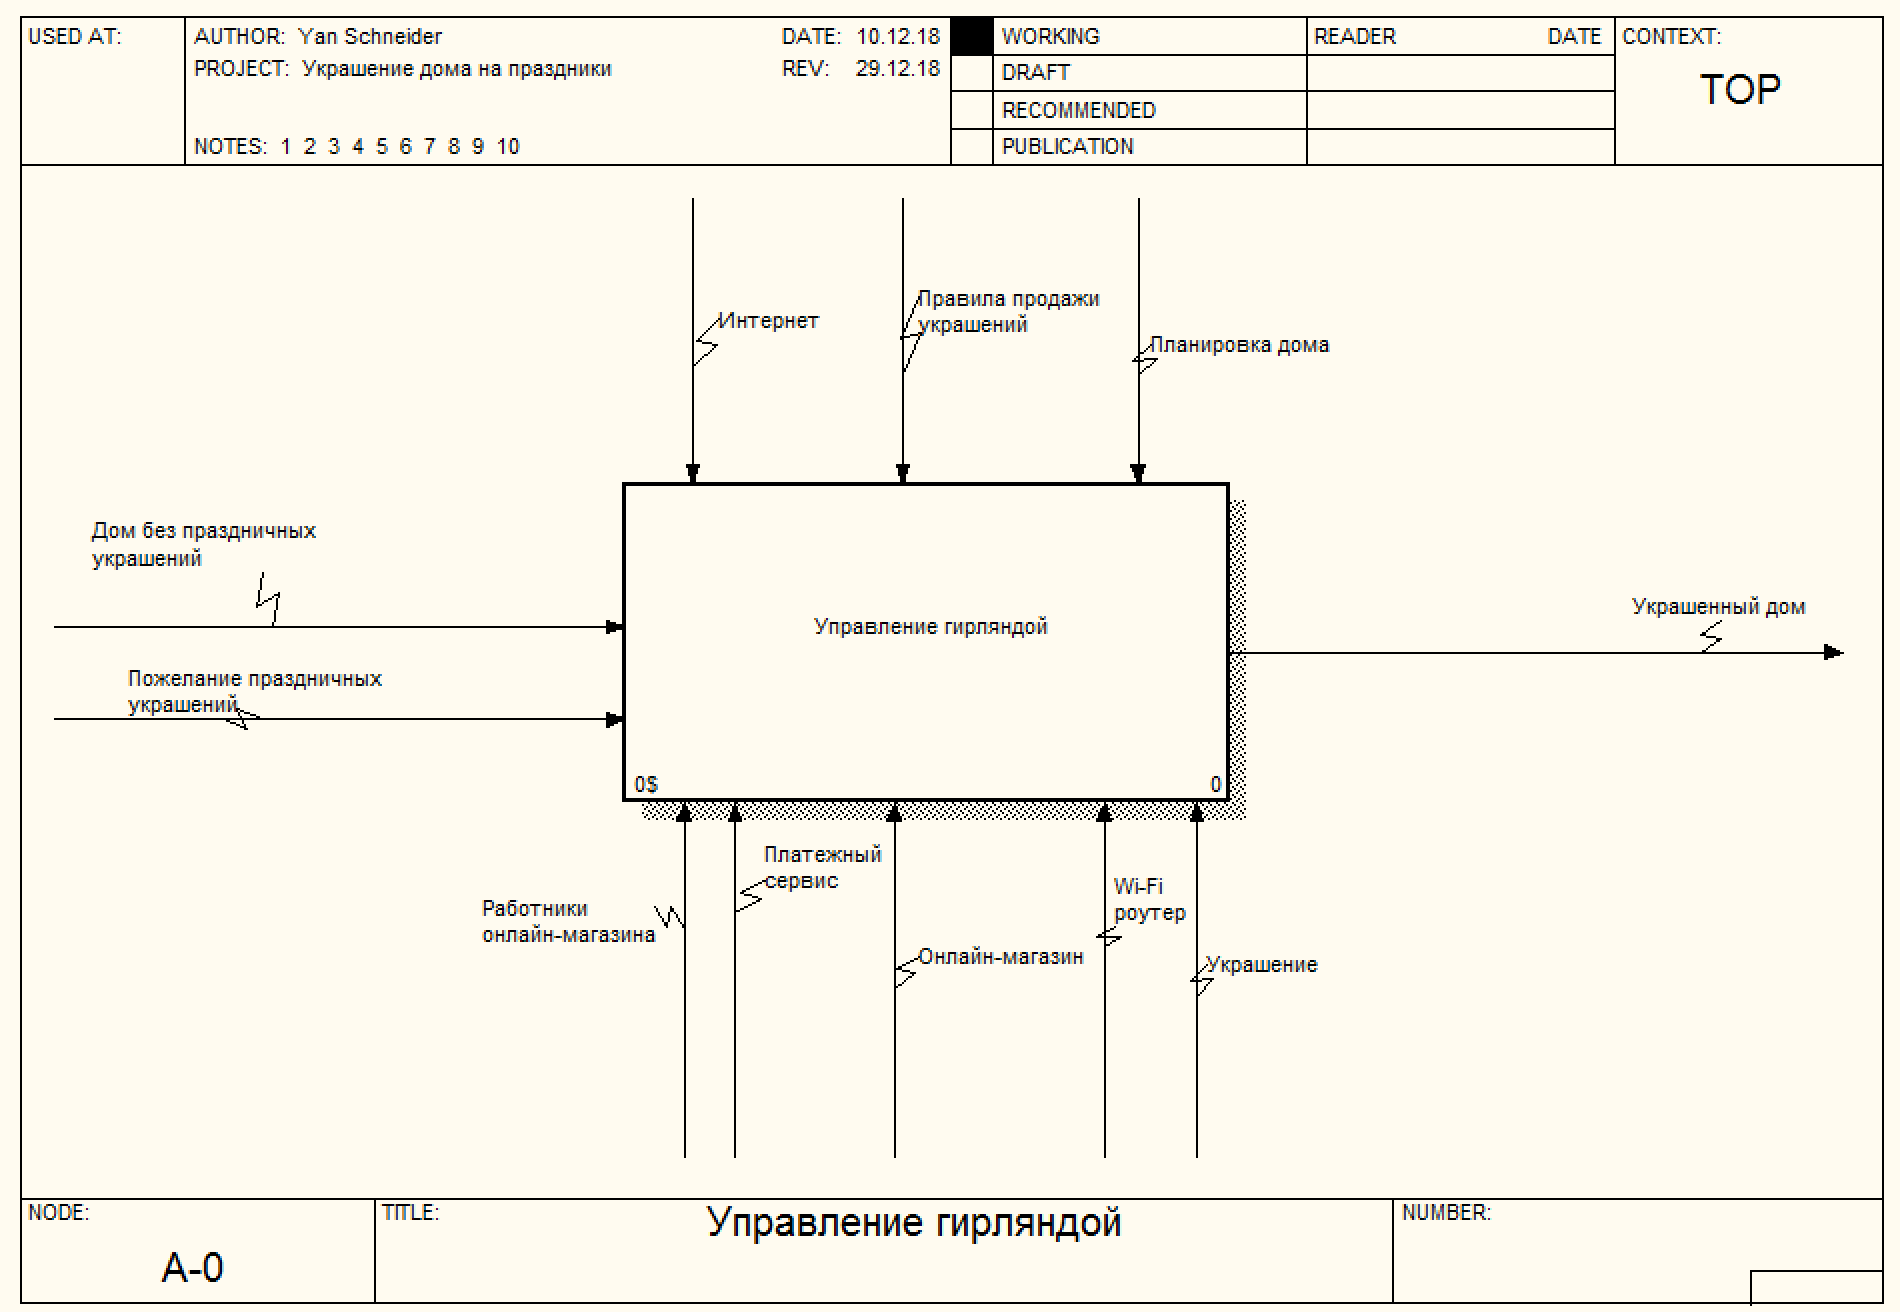
\includegraphics[scale=0.45]{figures/functionalModel/main.jpg}
	\caption{Контекстная диаграмма процесса управления гирляндой}
	\label{fig:develop:functionalModel:main}
\end{figure}

На рисунке~\ref{fig:develop:functionalModel:main} представлена контекстная диаграмма верхнего уровня, входными данными для которой являются дом без украшений и пожелания к ним. В рамках процесса на выходе получается украшенный дом. Далее в соответствии со вторым и третьим принципами, распишем основное действие на уровни.

Украшение дома декомпозировано на 4 блока: поиск, покупка, установка и настройка украшений.

Функциональная модель управления гирляндой показана на рисунке~\ref{fig:develop:functionalModel:a0_decoration}.

~
\begin{figure}[H]
\centering
	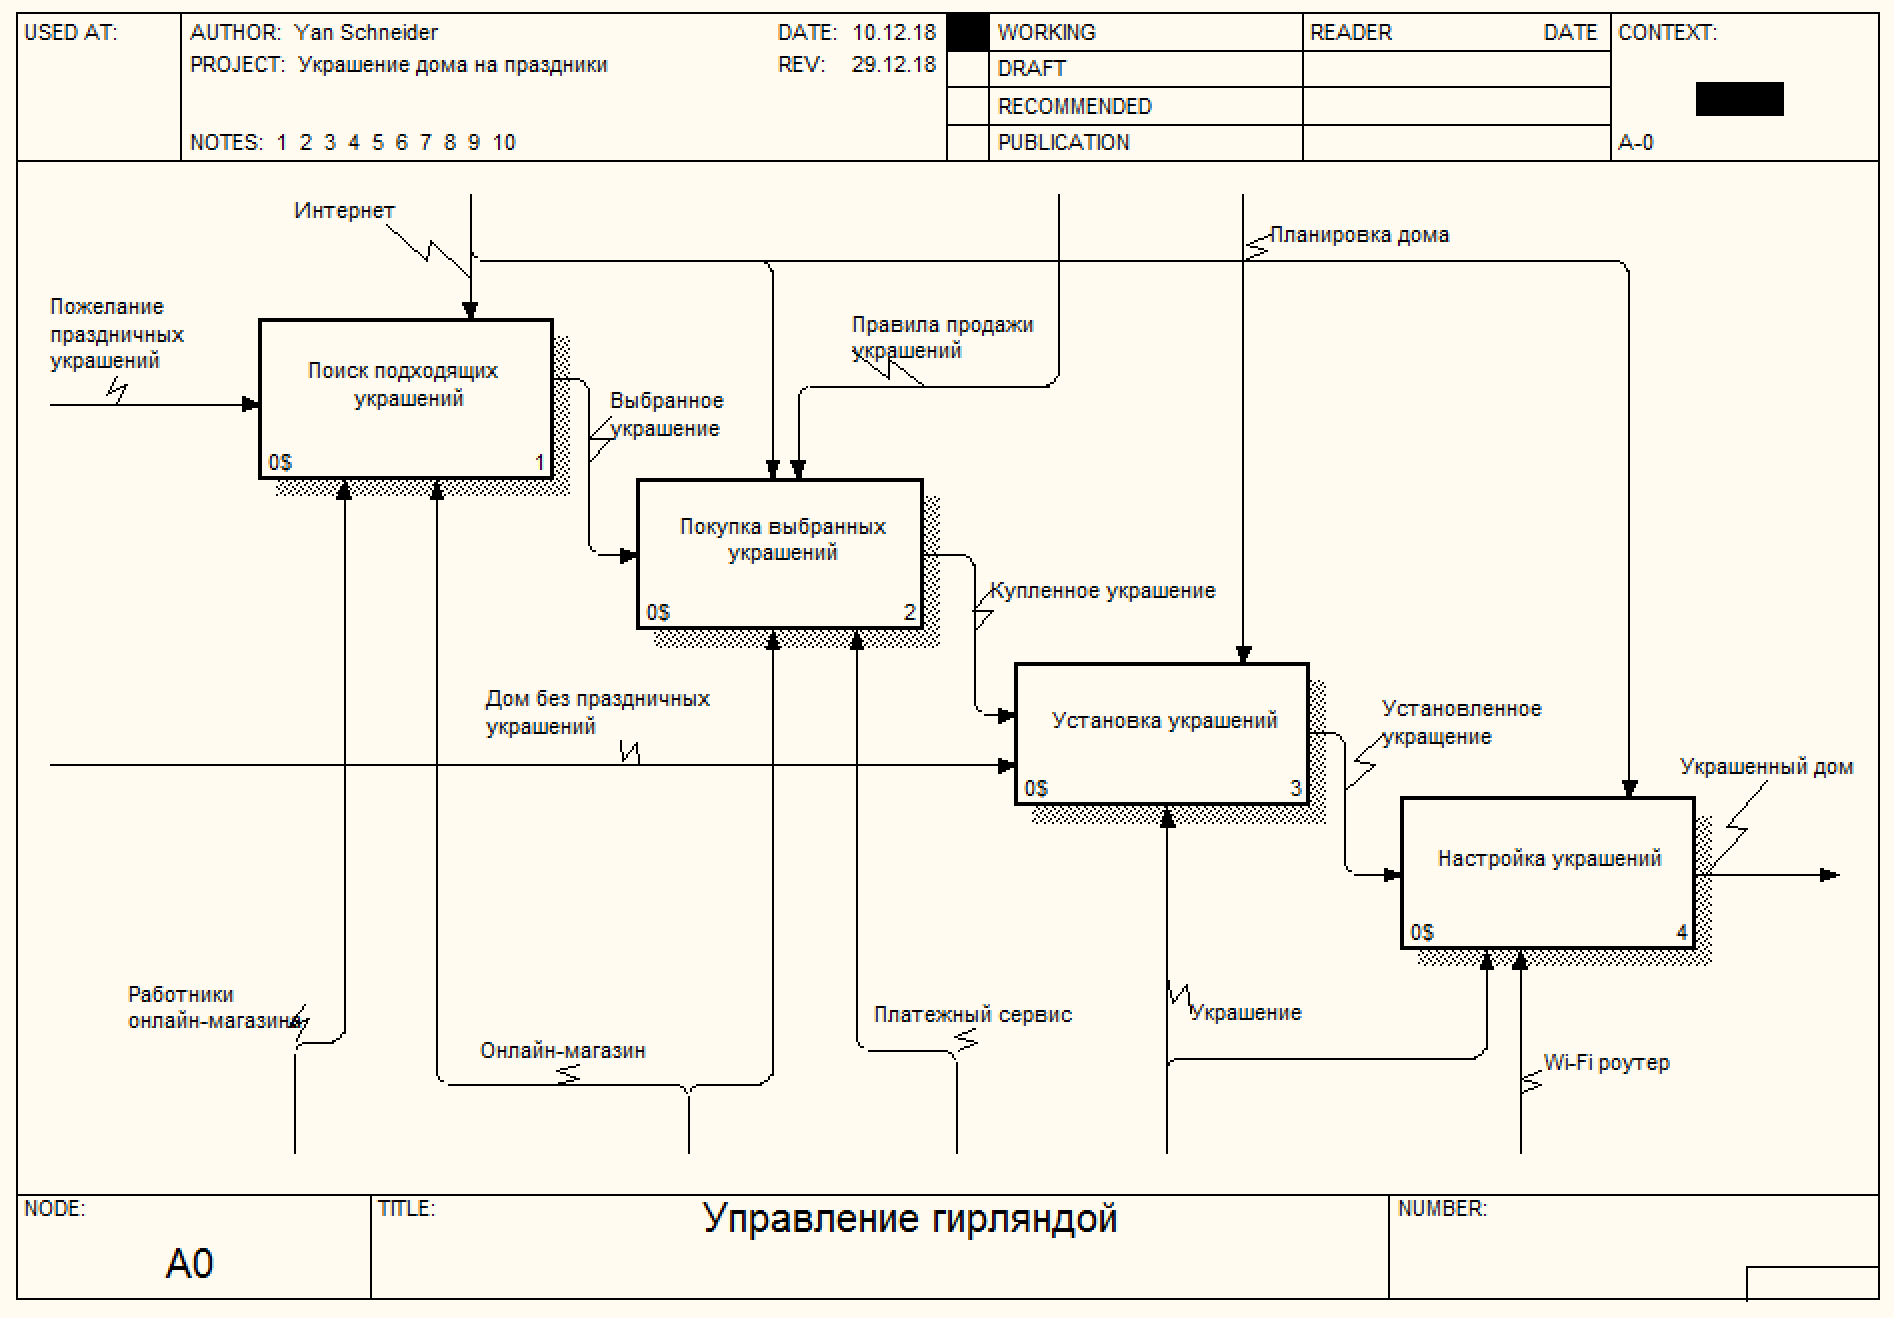
\includegraphics[scale=0.45]{figures/functionalModel/a0_decoration.jpg}
	\caption{Декомпозиция блока ``Управление гирляндой''}
	\label{fig:develop:functionalModel:a0_decoration}
\end{figure}

Рассмотрим последовательно каждый блок.

Первый блок (рисунок~\ref{fig:develop:functionalModel:a1_search}):

Данный блок необходим для поиска подходящего украшения для дома. Данный процесс включает в себя вход в онлайн магазин, установку фильтров для поиска, просмотр результатов поиска, консультация с работником онлайн-магазина (для дополнительной фильтрации списка выбранных украшений) и, наконец, выбор подходящего варианта.

 ~
\begin{figure}[H]
\centering
	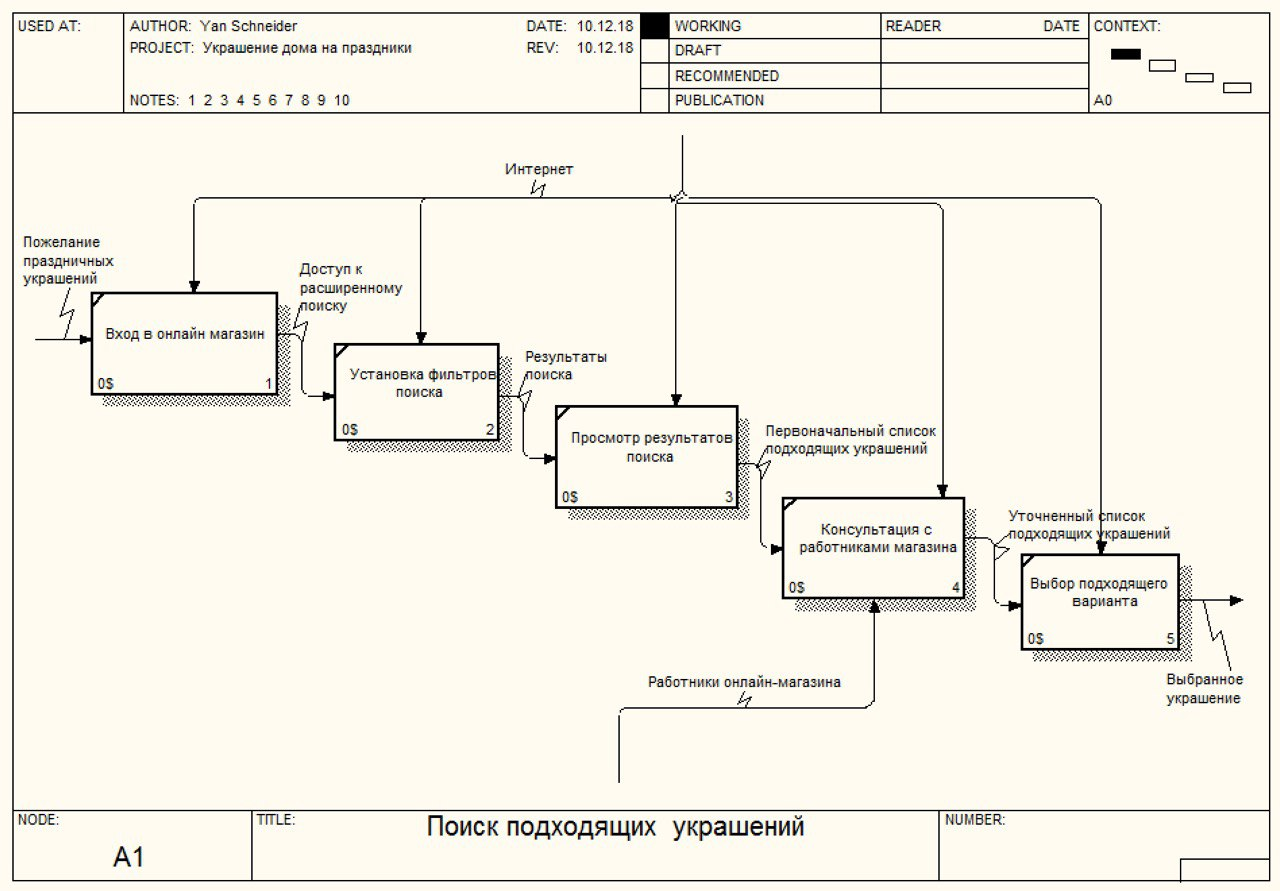
\includegraphics[scale=0.45]{figures/functionalModel/a1_search.jpg}
	\caption{Декомпозиция блока ``Поиск подходящих украшений''}
	\label{fig:develop:functionalModel:a1_search}
\end{figure}

Второй блок представлен на рисунке~\ref{fig:develop:functionalModel:a2_buy}. Данный блок включает в себя добавление заказа (украшения) в корзину, ввод платежной информации, ввод информации о доставке (адрес, индекс и т.д.) и оплата товара.

 ~
\begin{figure}[H]
\centering
	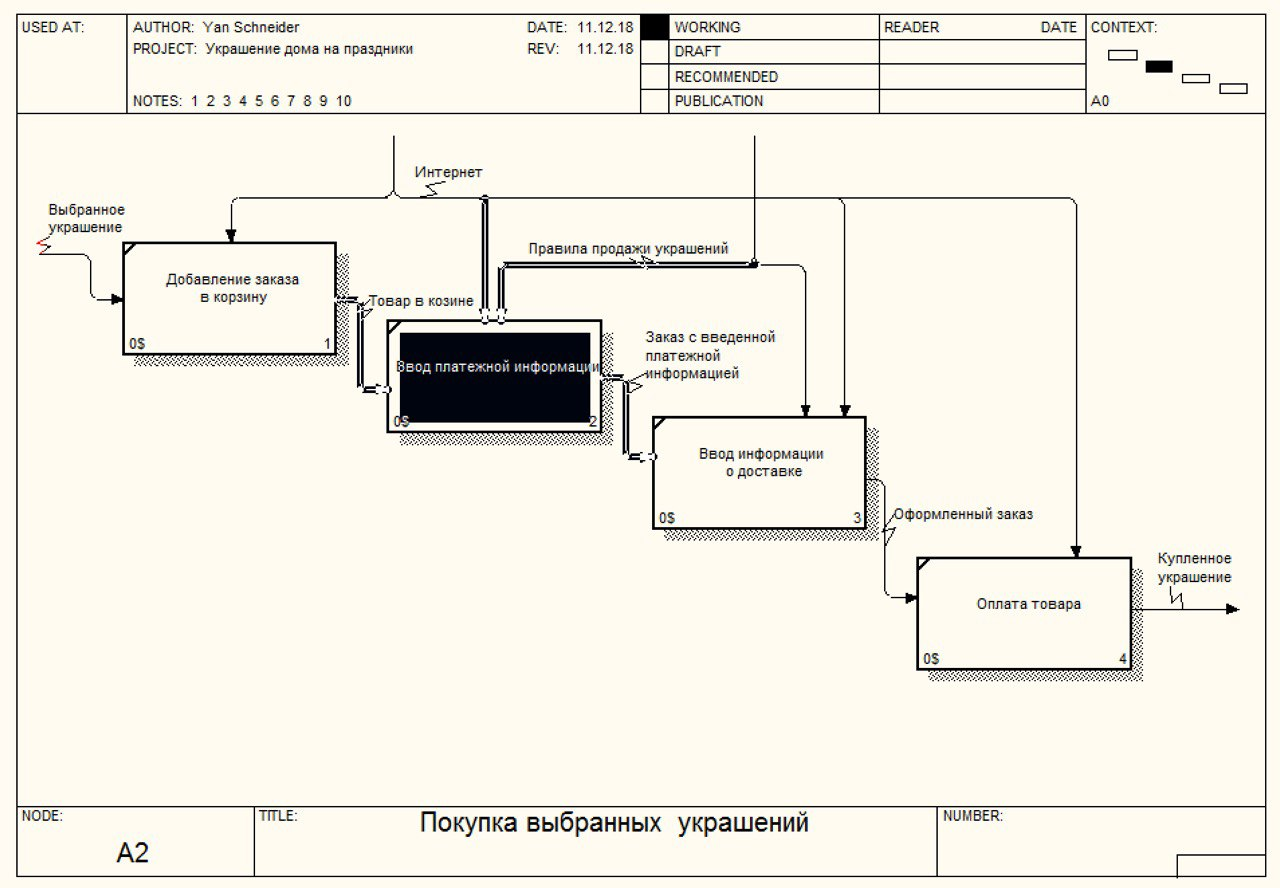
\includegraphics[scale=0.45]{figures/functionalModel/a2_buy.jpg}
	\caption{Декомпозиция блока ``Покупка выбранных украшений''}
	\label{fig:develop:functionalModel:a2_buy}
\end{figure}

 ~
\begin{figure}[H]
\centering
	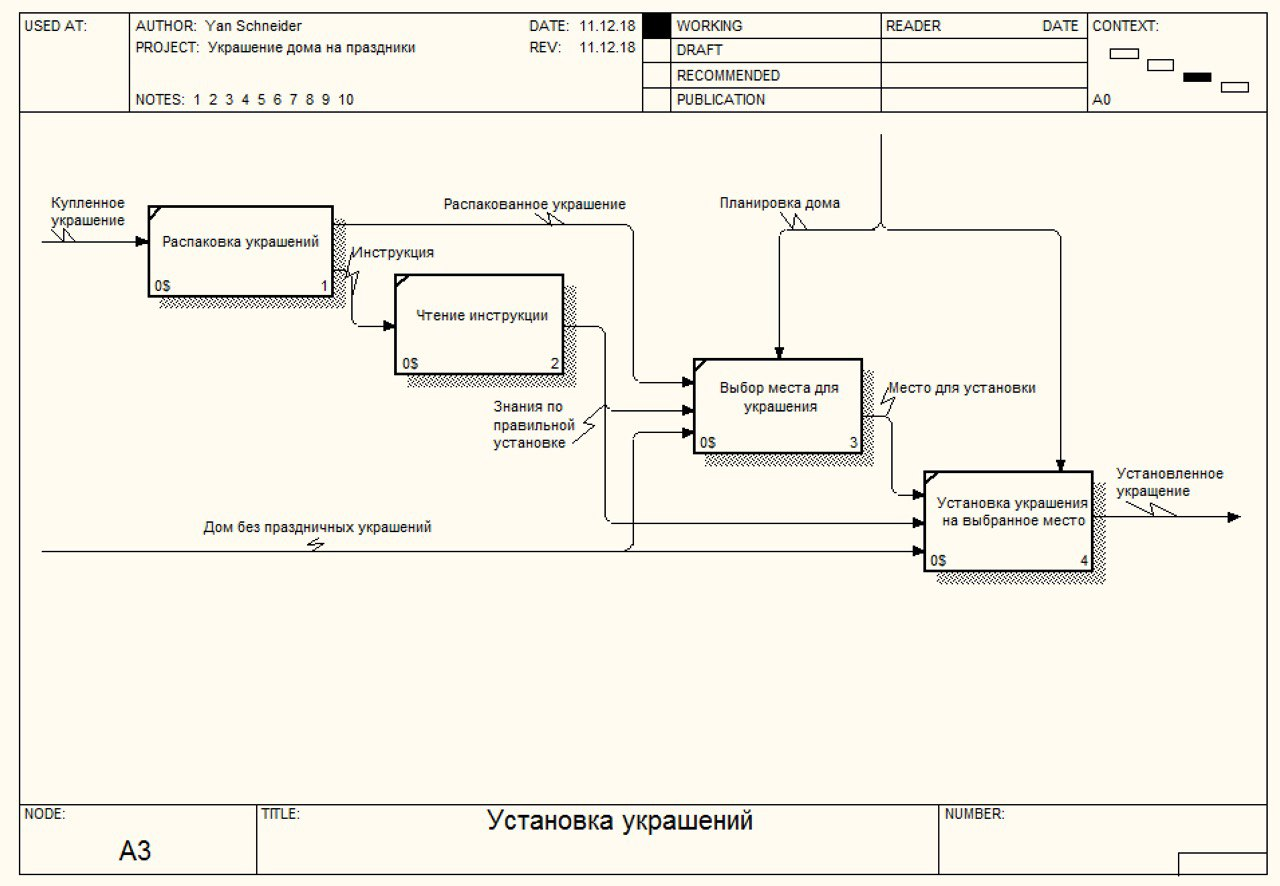
\includegraphics[scale=0.45]{figures/functionalModel/a3_install.jpg}
	\caption{Декомпозиция блока ``Установка украшений''}
	\label{fig:develop:functionalModel:a3_install}
\end{figure}

Третий блок (рисунок~\ref{fig:develop:functionalModel:a3_install}):

Данный блок описывает процесс установки купленного украшения в доме. Данный процесс включает в себя распаковку украшения, чтение инструкции, выбор места для украшения и его установка.

 ~
\begin{figure}[H]
\centering
	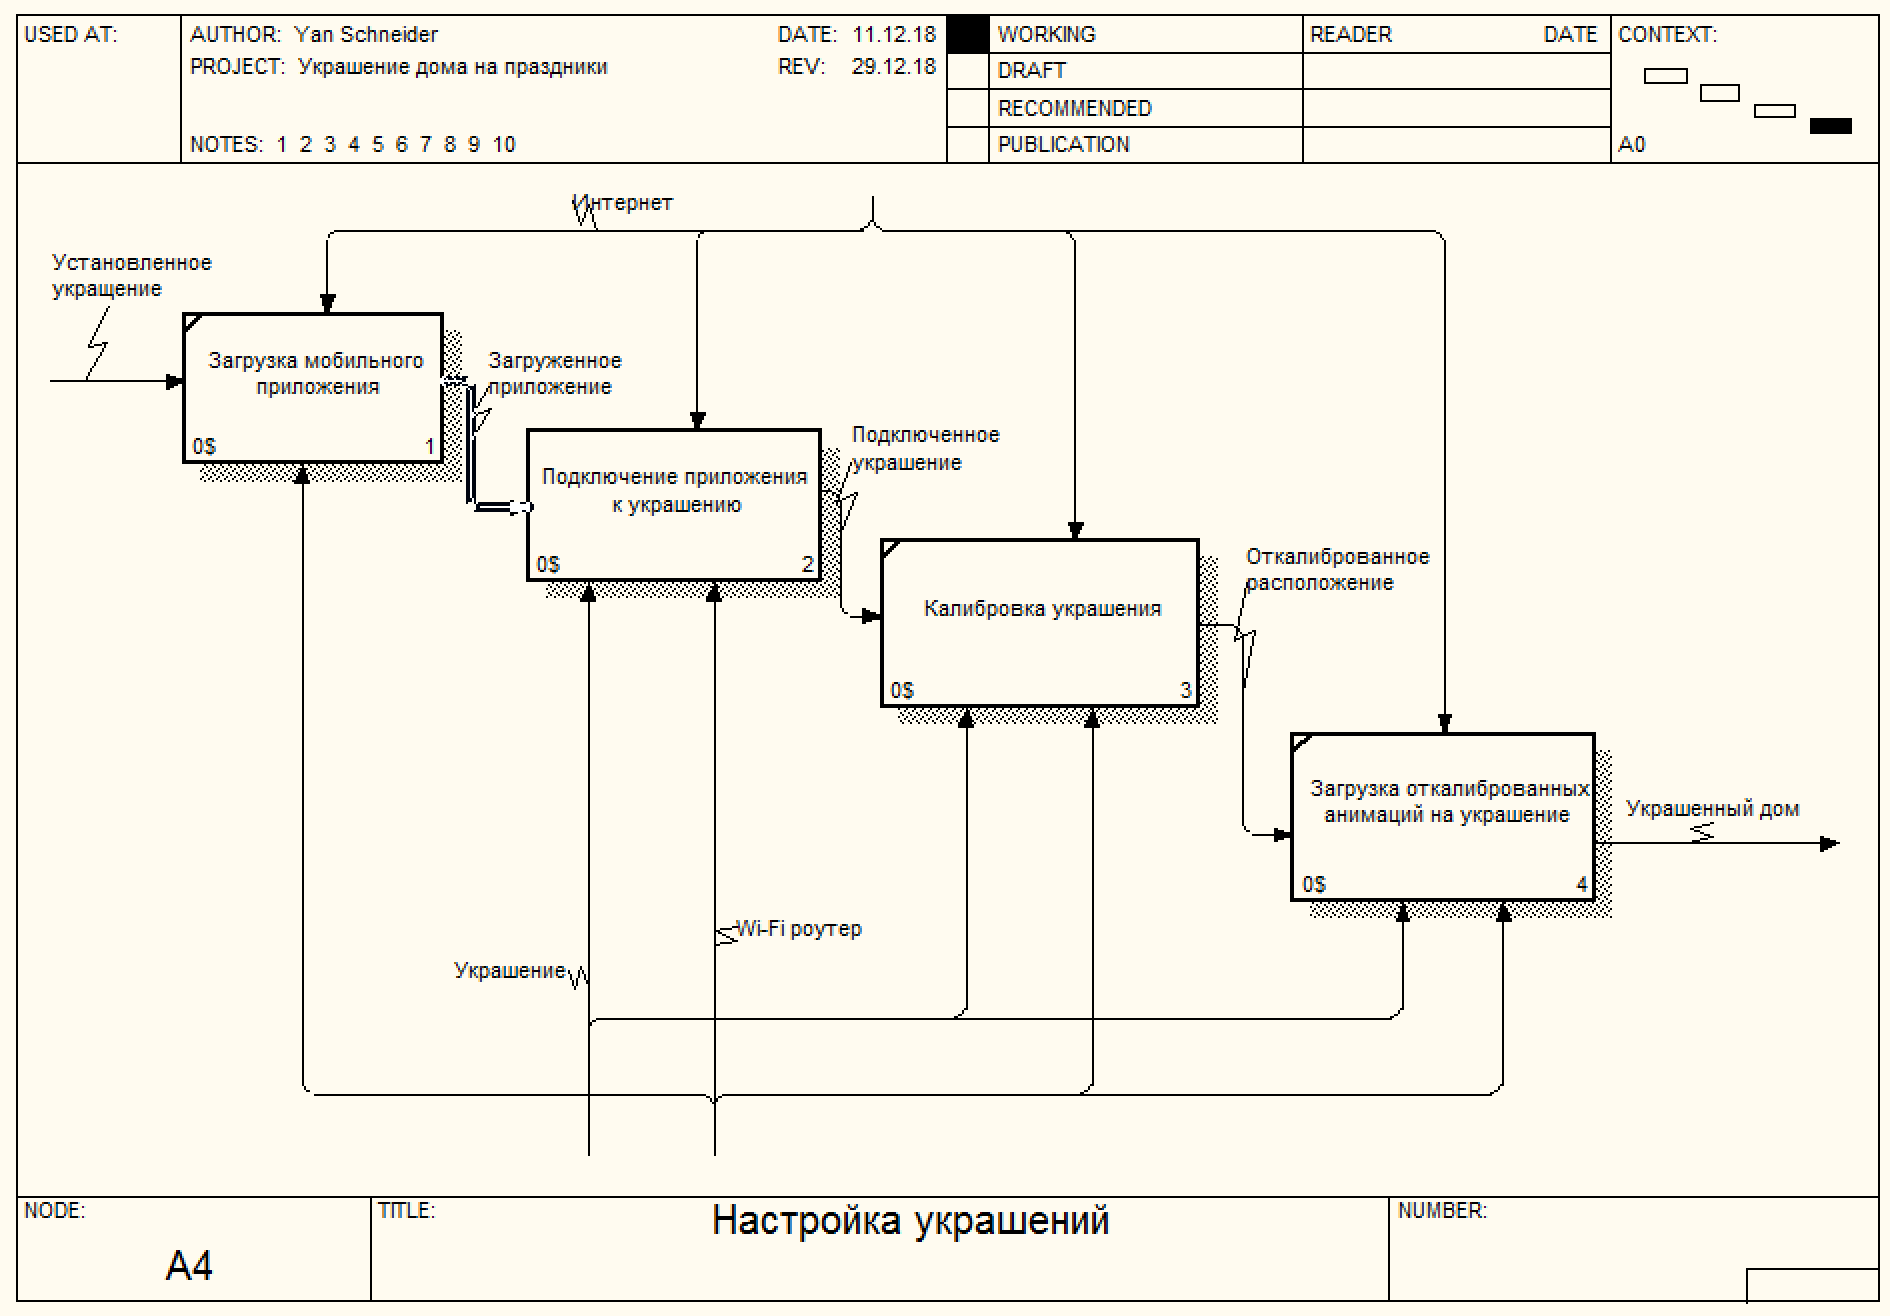
\includegraphics[scale=0.45]{figures/functionalModel/a4_settings.jpg}
	\caption{Декомпозиция блока ``Настройка украшений''}
	\label{fig:develop:functionalModel:a4_settings}
\end{figure}

Четвертый блок (рисунок~\ref{fig:develop:functionalModel:a4_settings}):

Данный блок описывает процесс настройки украшений. Данный процесс включает в себя загрузку приложения для управления украшениями, подключение их к приложению, калибровку и отправку уже откалиброванных анимаций на украшения. 

~
\begin{figure}[H]
\centering
	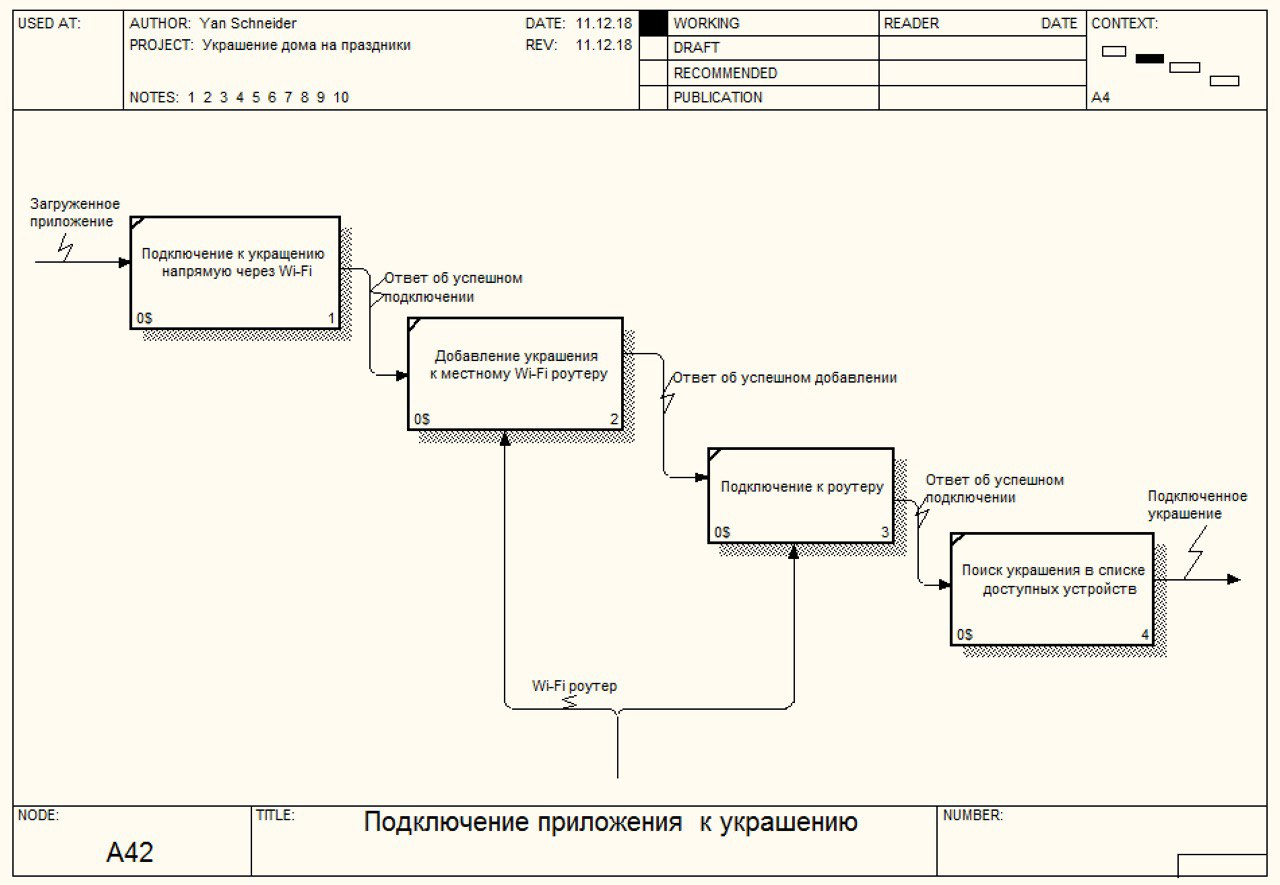
\includegraphics[scale=0.45]{figures/functionalModel/a42_connecting.jpg}
	\caption{Декомпозиция блока ``Подключение приложения к украшению''}
	\label{fig:develop:functionalModel:a42_connecting}
\end{figure}

Декомпозиция четвертого блока (рисунок~\ref{fig:develop:functionalModel:a42_connecting}):

Данная декомпозиция подробнее рассматривает процесс подключения мобильного приложения к украшению (украшениям). Она разбивает данный процесс на следующие компоненты: подключение напрямую к украшению через Wi-Fi, добавление украшения к местному роутеру (ввод пароля к точке). Затем идет процес подключения украшения к роутеру. После всего следует поиск украшения в списке доступных устройств.

\subsection{Разработка моделей представления системы}
\label{sec:develop:umlDiagrams}

\subsubsection{} Диаграмма вариантов использования
\label{sec:develop:umlDiagrams:useCase}

Диаграмма вариантов использования наглядно показывает взаимодействия актеров с системой. 

\subsubsection{} Диаграмма развертывания
\label{sec:develop:umlDiagrams:deployment}

Диаграмма развертывания необходима для представления того, какие устройства будут использовать те или иные компоненты. Из диаграммы понятно, что для использования данного продукта, пользователь должен иметь мобильный телефон под управлением операционной системы iOS (iPhone), а также нашу гирлянду. Для использования сетевых функций (через Firebase) нужно стабильное подключение к интернету (Рисунок~\ref{fig:develop:umlDiagrams:deployment}).

~
\begin{figure}[H]
\centering
	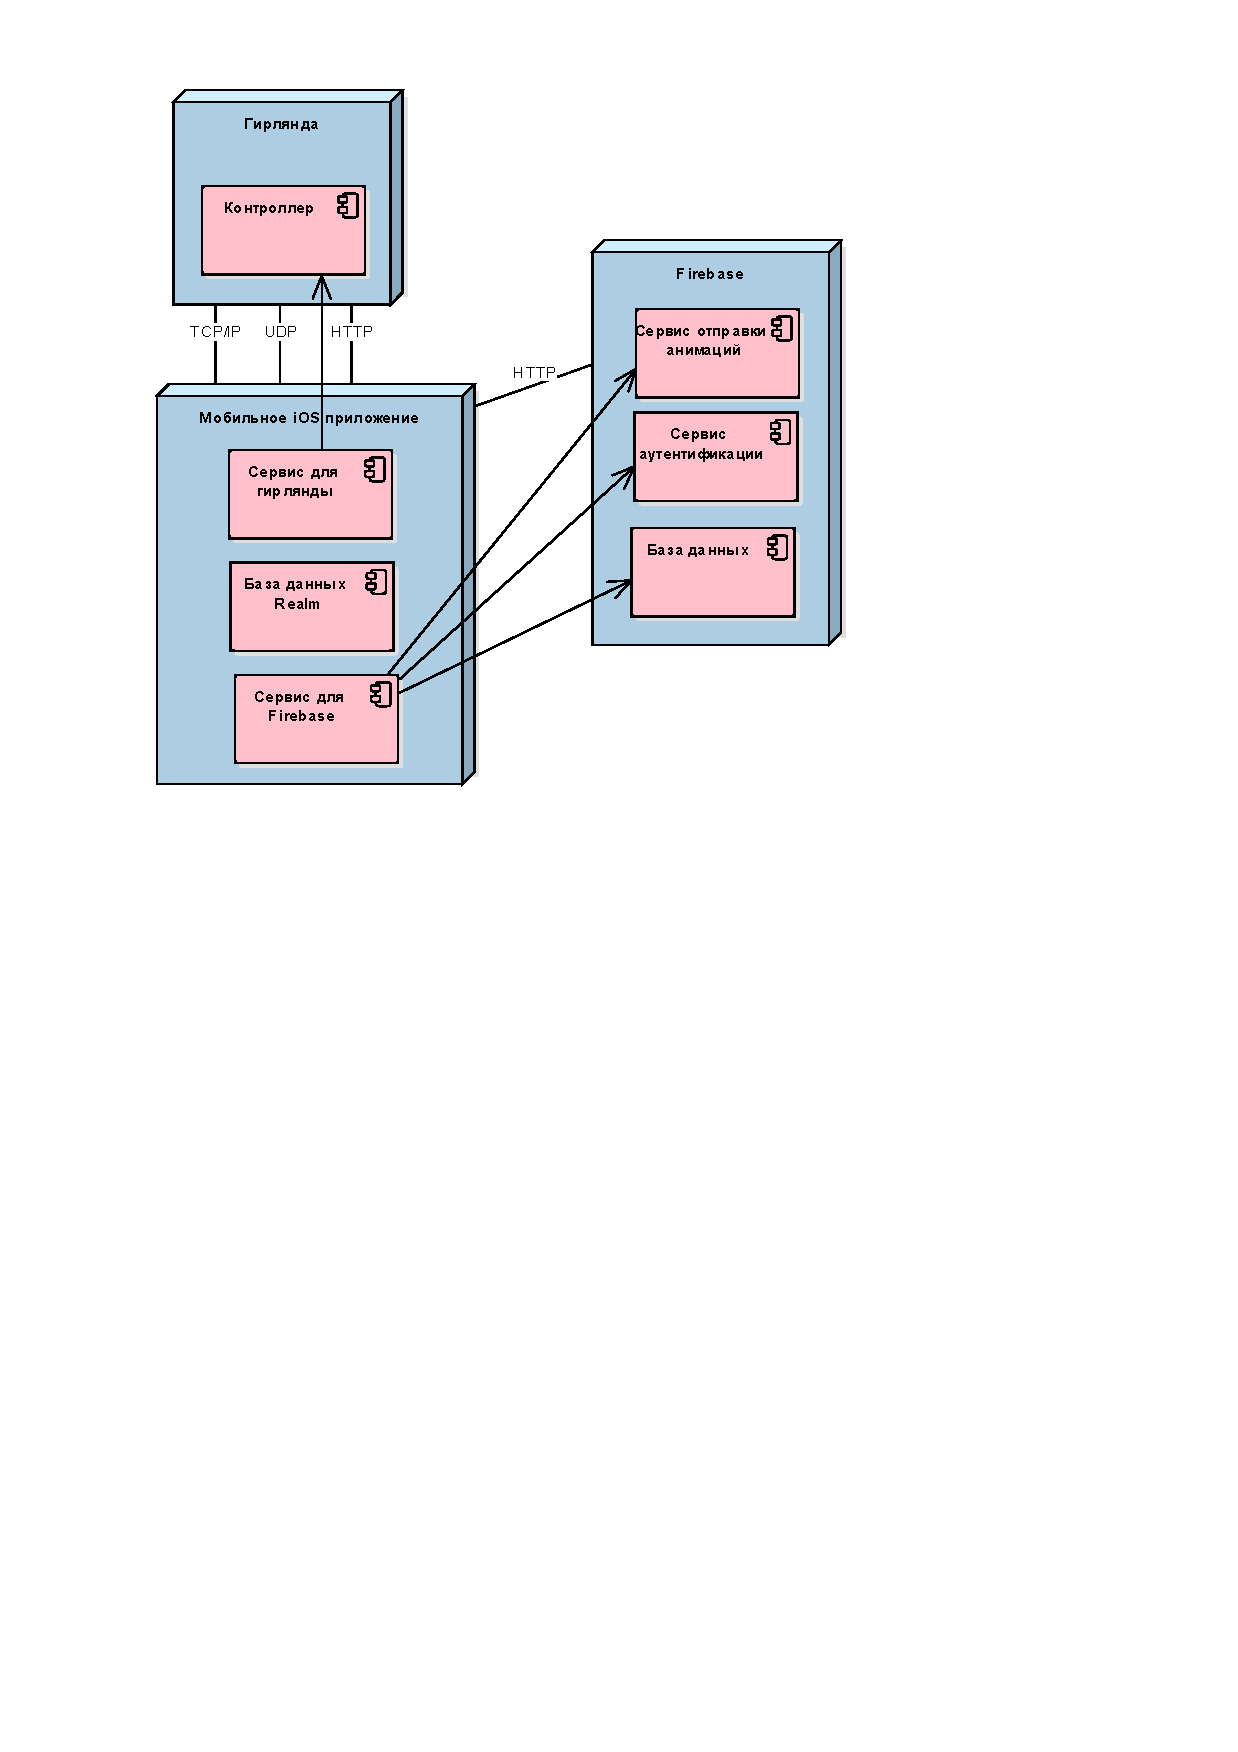
\includegraphics[scale=0.8]{figures/uml_deployment.pdf}
	\caption{Диаграмма системы для управления световым оборудованием}
	\label{fig:develop:umlDiagrams:deployment}
\end{figure}

\sectioncentered*{Заключение}
\addcontentsline{toc}{section}{Заключение}
%\setcounter{page}{74}
Предметной областью данного дипломного проекта является Интернет вещей и взаимодействие мобильных приложений с устройствами в нем. Во время создания данного дипломного проекта была изучена предметная область, рассмотрены уже существующие системы в Интернете вещей. Была разработана система калибровки адресных светодиодных лент для корректного отображения анимаций. Был проведен анализ деятельности предприятия ООО \enquote{Сампад}, а также рынка Internet of Things. Было предложено программное средство, которое позволяет не только управлять и создавать эффекты на гирляндах, но и обмениваться ими с другими пользователями. Было сделано технико-экономическое обоснование, рассчитаны затраты на разработку мобильного приложения и рассчитан экономический эффект.

В первой главе была изучена предметная область дипломного проекта. Было рассмотрено понятие Интернета вещей и его связь с мобильными приложениями. Был рассмотрен рынок IoT устройств в Беларуси и индустрия электронного светового оборудования. Также было представлено описание алгоритма распознавания расположения адресных светодиодных лент в пространстве.

Во второй главе был проведен аналих деятельности предприятия ООО \enquote{Сампад} и его участие в создании проектов в сфере IoT. Был освещен прогноз и сделана характеристика рынка IoT в 2019 году. Также было сделано описание бизнес-процесса приобретения и управления гирляндой.

В третьей главе были подробно описаны все аспекты разработки программного обеспечение, а именно мобильного приложения для управления адресными светодиодными лентами. Были разработаны информационная модель и модели представления системы. Был обоснован выбор языка программирования, а также некоторых архитектурных аспектов. Также были описаны некоторые алгоритмы системы.

Следующая основная цель -- внедрение и популяризация программного средства среди пользователей. Параллельно с этим будет производиться дальнейшая его разработка. Будет внедрена поддержка гирлянд с различным количеством лампочек (150 и 350). Будет развиваться алгоритм калибровки. Кроме того, будут добавляться новые анимации.


% Зачем: Изменение надписи для списка литературы
% Почему: Пункт 2.8.1 Требований по оформлению пояснительной записки.
\renewcommand{\bibsection}{\sectioncentered*{Cписок использованных источников}}
\phantomsection\pagebreak % исправляет нумерацию в документе и исправляет гиперссылки в pdf
\addcontentsline{toc}{section}{Cписок использованных источников}

% Зачем: включить в список литературы все источники из базы (даже если на них нет ссылок в тексте).
% \nocite{*}

% Зачем: Печать списка литературы. База данных литературы - файл bibliography.bib
\bibliography{content/main/bibliography.bib}

\newpage


% Appendices

\BeginAppendices

\appendice{Диаграмма последовательности системы}
\label{app:sequence}

~
\begin{figure}[H]
\centering
	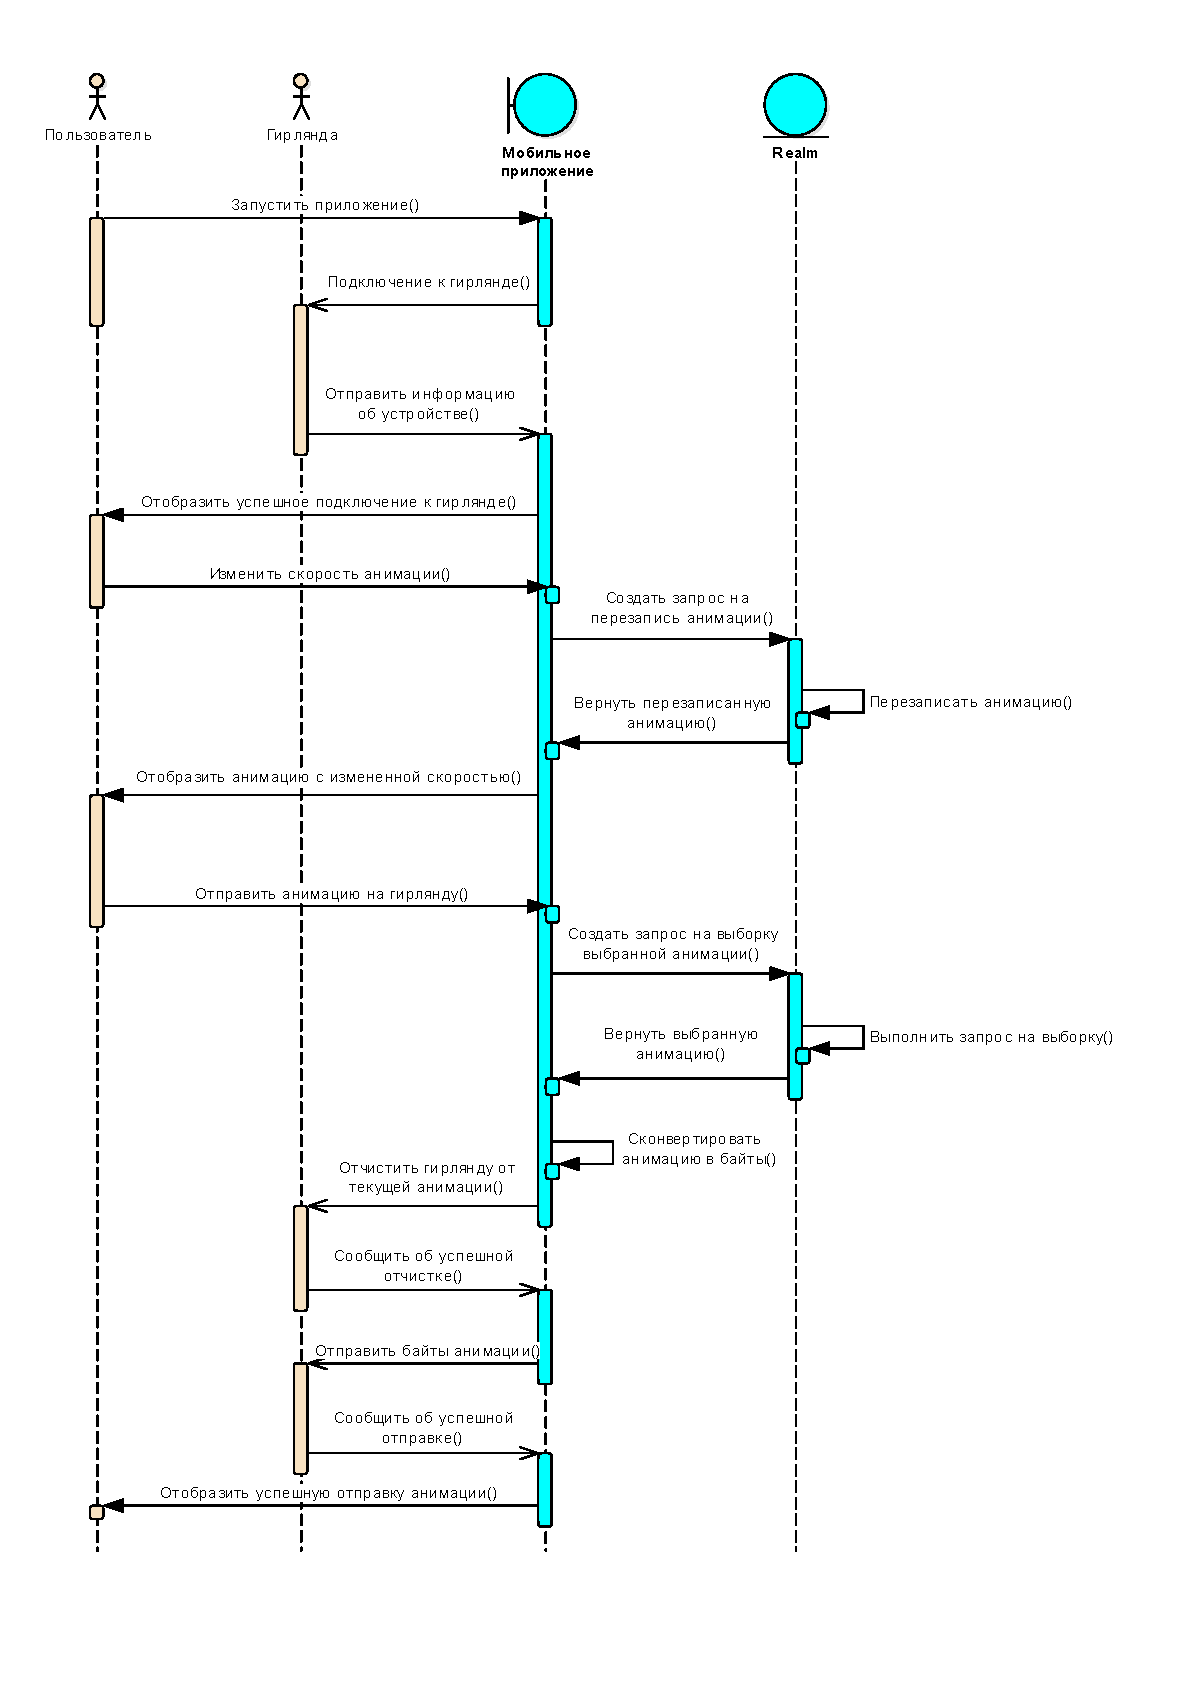
\includegraphics[scale=0.8]{figures/uml_sequence.pdf}
	\caption{Диаграмма последовательностей процесса редактирования и отправки анимации}
	\label{fig:appendices:sequence}
\end{figure}

\appendice{Диаграмма информационной модели системы}
\label{app:er}

~
\begin{figure}[H]
\centering
	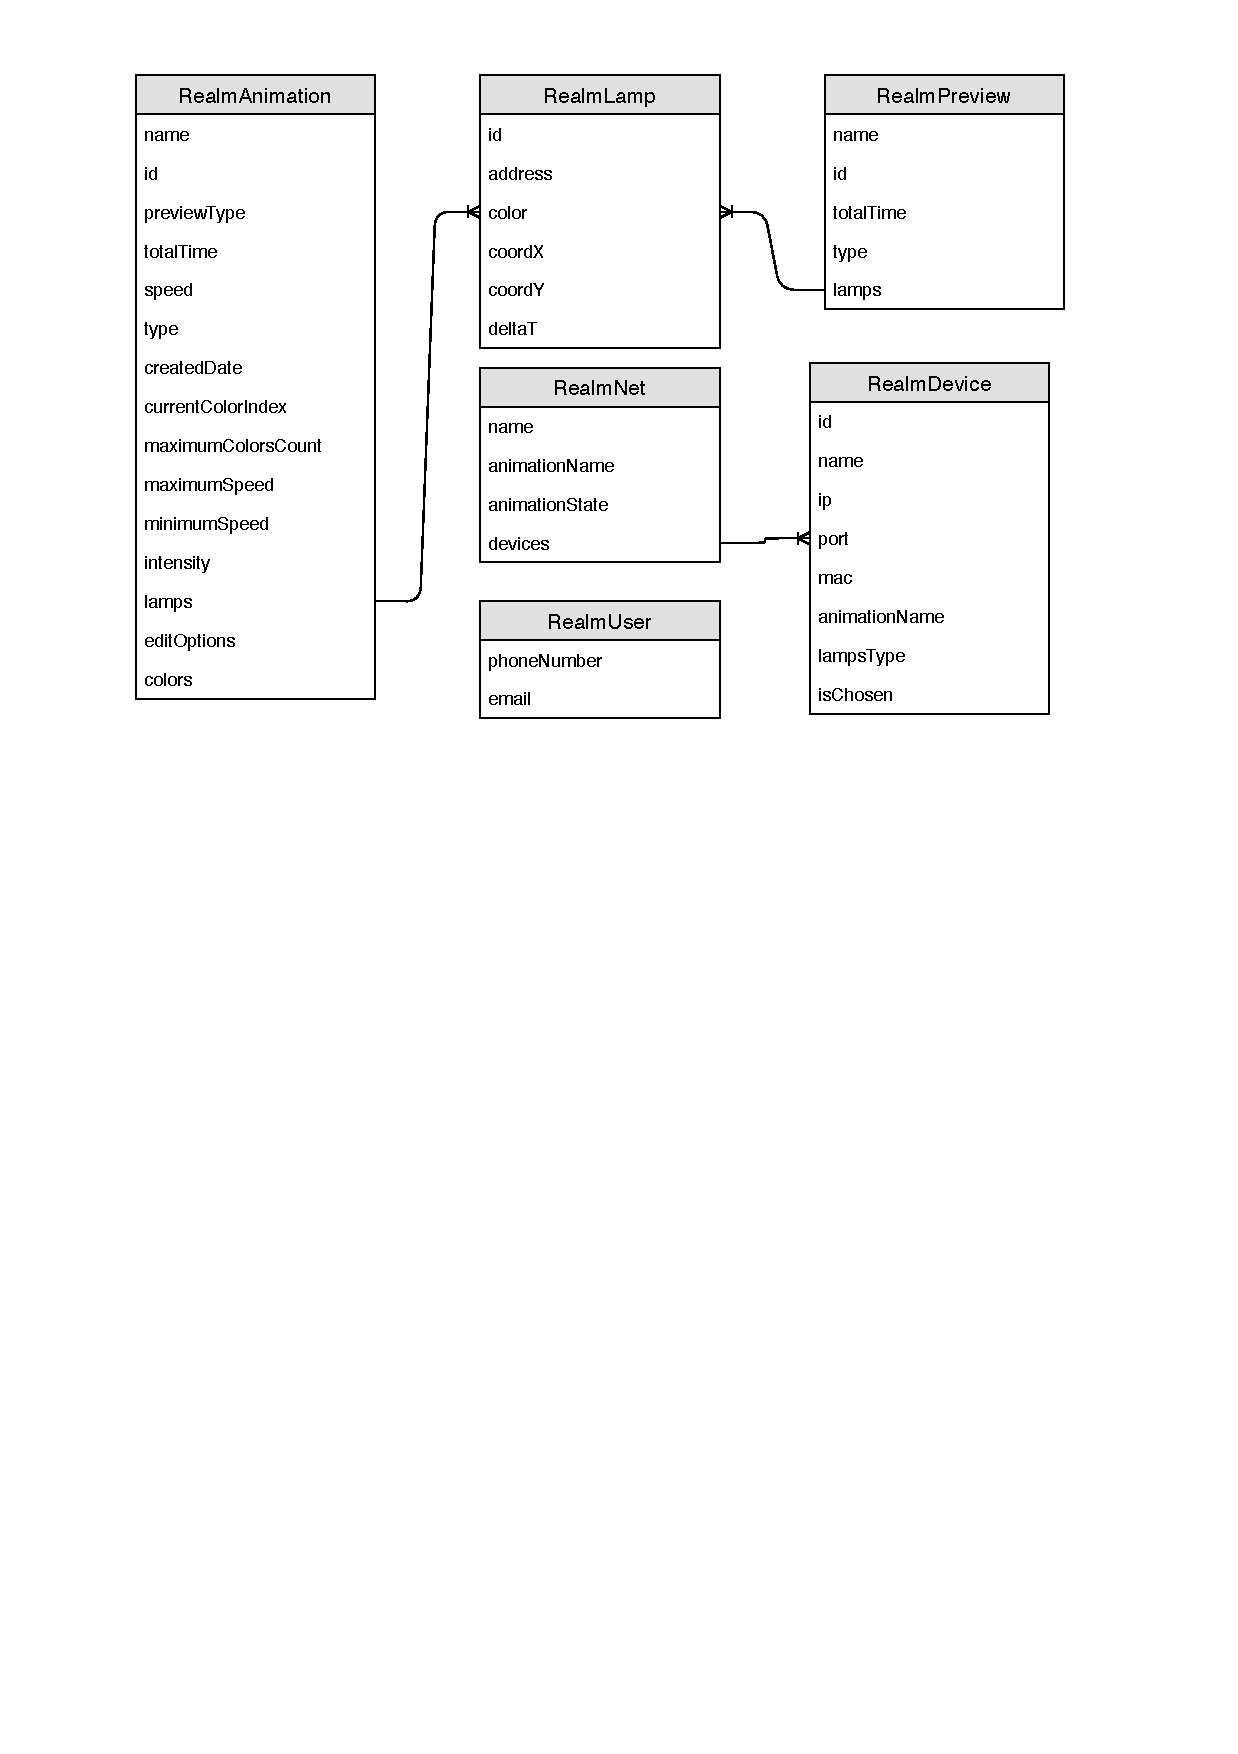
\includegraphics[scale=0.8]{figures/er_diagram.pdf}
	\caption{Информационная модель системы}
	\label{fig:appendices:er}
\end{figure}


\end{document}
